% !TeX program = pdflatex
% !TeX encoding = UTF-8
% =============================================================================
%  PLANTILLA — Presentación Beamer con Tema UNAM
%  Maestría en Urbanismo, UNAM – FES Acatlán
%  Versión 1.0 — Noviembre 2027
%
%  USO:
%    1. Edita el bloque "PERSONALIZACIÓN" con los datos de tu presentación.
%    2. Edita los colores en Latex/BeamerTheme.tex (sección PALETA DE COLORES).
%    3. Completa las secciones en /secciones/ con tu contenido.
%    4. Compila con: pdflatex → bibtex → pdflatex → pdflatex
% =============================================================================

\documentclass[aspectratio=169, 12pt]{beamer}

% ═════════════════════════════════════════════════════════════════════════════
%  PERSONALIZACIÓN — Edita solo esta sección para cada nueva presentación
% ═════════════════════════════════════════════════════════════════════════════
\newcommand{\TituloPresent}{El aula como entorno inmersivo}
\newcommand{\SubtituloPresent}{Experiencia sensorial y cognitiva del autismo}
\newcommand{\Autor}{Hernán Galileo Cabrera Garibaldi}
\newcommand{\MateriaCorta}{Didáctica — Semestre 2027-1}   % Aparece en el pie
\newcommand{\ProfesorAsignado}{Dra. Lorena Beatriz Garces Zepeda}
\newcommand{\Semestre}{2027-1}
\newcommand{\ProgramaCorto}{Maestría y Doctorado en Urbanismo}
\newcommand{\Facultad}{FES Acatlán}
\newcommand{\FechaPresent}{Naucalpan, 2027-1}
% ═══════════════════════════════════════════════════════════════════════════──

% Metadatos de Beamer (usa las variables de arriba)
\title{\TituloPresent}
\subtitle{\SubtituloPresent}
\author{\Autor}
\date{\FechaPresent}

% =============================================================================
%  TEMA Y PAQUETES — cargados desde Latex/BeamerTheme.tex
% =============================================================================
% =============================================================================
%  BeamerTheme.tex — Tema personalizado para presentaciones académicas
%  Maestría en Urbanismo, UNAM – FES Acatlán
%
%  NOTA: Incluido desde main.tex con % =============================================================================
%  BeamerTheme.tex — Tema personalizado para presentaciones académicas
%  Maestría en Urbanismo, UNAM – FES Acatlán
%
%  NOTA: Incluido desde main.tex con % =============================================================================
%  BeamerTheme.tex — Tema personalizado para presentaciones académicas
%  Maestría en Urbanismo, UNAM – FES Acatlán
%
%  NOTA: Incluido desde main.tex con \input{Latex/BeamerTheme}
%        en el preámbulo, después de \documentclass{beamer}.
% =============================================================================


% ═════════════════════════════════════════════════════════════════════════════
%  PALETA DE COLORES
%  El tema se carga desde Latex/color-config.tex → Latex/Colores/<tema>.tex
%  Temas disponibles: Institucional | Teal | VerdeOlivo | Purpura | Rojo
%
%  Cambiar el color de esta presentación:
%    • Permanente: edita \providecommand en Latex/color-config.tex
%    • Una compilación: make Presentacion DIR=<ruta> COLOR=Teal
% ═════════════════════════════════════════════════════════════════════════════
\usepackage{xcolor}
\input{Latex/color-config}            % define \ColorTema (default: Institucional)
\input{Latex/Colores/\ColorTema}      % carga ColorPrincipal y ColorAcento
\definecolor{ColorFondo}    {RGB}{248, 250, 255}  % Blanco azulado suave
\definecolor{ColorTexto}    {RGB}{20,  20,  20}   % Casi negro
\definecolor{ColorAlerta}   {RGB}{183, 28,  28}   % Rojo de énfasis
% ═════════════════════════════════════════════════════════════════════════════


% =============================================================================
%  1. IDIOMA, CODIFICACIÓN Y TIPOGRAFÍA
% =============================================================================
\usepackage[utf8]{inputenc}
\usepackage[T1]{fontenc}
\usepackage[spanish,es-tabla,es-nodecimaldot]{babel}
\usepackage{csquotes}
\usepackage{microtype}
\usepackage{lmodern}       % Fuente Latin Modern — mejor calidad que CM


% =============================================================================
%  2. TEMA BASE Y PERSONALIZACIÓN DE COLORES
% =============================================================================
\usetheme{Madrid}

% Sobreescribir paleta de Madrid con ColorPrincipal
\setbeamercolor{palette primary}   {bg=ColorPrincipal, fg=white}
\setbeamercolor{palette secondary} {bg=ColorPrincipal!85!black, fg=white}
\setbeamercolor{palette tertiary}  {bg=ColorPrincipal!70!black, fg=white}
\setbeamercolor{palette quaternary}{bg=ColorPrincipal, fg=white}
\setbeamercolor{structure}         {fg=ColorPrincipal}

% Título y frame titles
\setbeamercolor{title}      {fg=white, bg=ColorPrincipal}
\setbeamercolor{frametitle} {fg=white, bg=ColorPrincipal}

% Bloque estándar
\setbeamercolor{block title}{fg=white, bg=ColorPrincipal}
\setbeamercolor{block body} {fg=ColorTexto, bg=ColorFondo}

% Bloque de alerta
\setbeamercolor{block title alerted}{fg=white, bg=ColorAlerta}
\setbeamercolor{block body alerted} {fg=ColorTexto, bg=ColorFondo}

% Bloque de ejemplo
\setbeamercolor{block title example}{fg=white, bg=ColorPrincipal!60!black}
\setbeamercolor{block body example} {fg=ColorTexto, bg=ColorFondo}

% Acento en texto de énfasis
\setbeamercolor{alerted text}{fg=ColorAcento!80!black}

% Itemize bullets
\setbeamercolor{item}{fg=ColorPrincipal}
\setbeamercolor{subitem}{fg=ColorAcento!80!black}


% =============================================================================
%  3. PERSONALIZACIÓN DE FOOTLINE (pie de diapositiva)
%     Madrid genera: [Autor | Título] [Sección] [N/Total]
%     Aquí se redefine para mostrar: [Autor] | [Materia] | [N/Total]
% =============================================================================
\makeatletter
\setbeamertemplate{footline}{%
  \leavevmode%
  \hbox{%
    \begin{beamercolorbox}[wd=.45\paperwidth, ht=2.5ex, dp=1.5ex, leftskip=0.4cm]{palette primary}%
      \usebeamerfont{author in head/foot}\insertshortauthor
    \end{beamercolorbox}%
    \begin{beamercolorbox}[wd=.40\paperwidth, ht=2.5ex, dp=1.5ex, center]{palette secondary}%
      \usebeamerfont{title in head/foot}\MateriaCorta
    \end{beamercolorbox}%
    \begin{beamercolorbox}[wd=.15\paperwidth, ht=2.5ex, dp=1.5ex, rightskip=0.4cm, right]{palette primary}%
      \usebeamerfont{date in head/foot}%
      \insertframenumber{} / \inserttotalframenumber
    \end{beamercolorbox}%
  }%
  \vskip0pt%
}
\makeatother


% =============================================================================
%  4. HEADLINE — eliminado: la sección se muestra dentro del frametitle
% =============================================================================
\setbeamertemplate{headline}{}


% =============================================================================
%  5. FRAMETITLE — DOS VARIANTES
%     La sección activa se muestra como etiqueta pequeña dentro del cuadro azul,
%     encima del título principal. Elimina el efecto de "doble barra" anterior.
%
%     Default (\begin{frame}{título}): cuadro azul unificado.
%     Con línea dorada: escribe \framelinea justo antes de \begin{frame}.
% =============================================================================
\usepackage{etoolbox}

% Variante 1 (default): cuadro azul, centrado con sep
\defbeamertemplate{frametitle}{simple}{%
  \begin{beamercolorbox}[wd=\paperwidth, sep=0.20cm, left, leftskip=0.20cm]{frametitle}%
    {\tiny\color{white!60!ColorPrincipal}\insertsectionhead}\\[-0.05cm]%
    \bfseries\insertframetitle\strut%
  \end{beamercolorbox}%
}

% Variante 2: cuadro azul + línea dorada debajo
\defbeamertemplate{frametitle}{conlinea}{%
  \begin{beamercolorbox}[wd=\paperwidth, sep=0.20cm, dp=0cm, left, leftskip=0.20cm]{frametitle}%
    {\tiny\color{white!60!ColorPrincipal}\insertsectionhead}\\[-0.05cm]%
    \bfseries\insertframetitle\strut%
  \end{beamercolorbox}%
  \vspace{-0.06cm}%
  {\color{ColorAcento}\rule{\paperwidth}{2.5pt}}%
}

% Activar variante simple como default
\setbeamertemplate{frametitle}[simple]

% Flag interno
\newif\ifusarlineadorada
\usarlineadoradafalse

% Al abrir cada frame: aplica la variante correcta y reinicia el flag
\AtBeginEnvironment{frame}{%
  \ifusarlineadorada
    \setbeamertemplate{frametitle}[conlinea]%
    \global\usarlineadoradafalse
  \else
    \setbeamertemplate{frametitle}[simple]%
  \fi
}

% \framelinea — úsalo justo antes de \begin{frame} para activar la línea dorada
%   Ejemplo:
%     \framelinea
%     \begin{frame}{Mi Título Destacado}
%       ...
%     \end{frame}
\newcommand{\framelinea}{\global\usarlineadoradatrue}


% =============================================================================
%  6. PÁGINA DE TÍTULO PERSONALIZADA
% =============================================================================
\setbeamertemplate{title page}{%
  \begin{center}
    \vspace{0.2cm}
    % ── Escudos + texto institucional ────────────────────────────────────────
    \noindent%
    \begin{minipage}[c]{0.13\textwidth}
      \centering
      \includegraphics[height=1.3cm]{UNAM_crest_blue.pdf}
    \end{minipage}%
    \begin{minipage}[c]{0.72\textwidth}
      \centering
      {\tiny\textbf{UNIVERSIDAD NACIONAL AUTÓNOMA DE MÉXICO}}\\[0.05cm]
      {\tiny\textbf{\ProgramaCorto}}\\[0.05cm]
      {\tiny\textbf{\Facultad}}
    \end{minipage}%
    \begin{minipage}[c]{0.13\textwidth}
      \centering
      \includegraphics[height=1.3cm]{escudo-fes-azul.png}
    \end{minipage}

    \vspace{0.15cm}
    {\color{ColorAcento}\rule{0.85\textwidth}{1.5pt}}
    \vspace{0.3cm}

    {\large\bfseries\color{ColorPrincipal}\inserttitle}\\[0.3cm]
    {\small\color{ColorPrincipal}\insertsubtitle}

    \vspace{0.5cm}
    {\color{ColorAcento}\rule{0.5\textwidth}{0.8pt}}
    \vspace{0.3cm}

    {\small\textbf{\insertauthor}}\\[0.15cm]
    {\scriptsize PROFESOR ASIGNADO: \ProfesorAsignado}\\[0.1cm]
    {\scriptsize SEMESTRE: \Semestre}

    \vfill
    {\scriptsize\insertdate}
  \end{center}
}


% =============================================================================
%  7. DIAPOSITIVA DE SECCIÓN
%     Solo aparece a partir de la SEGUNDA sección.
%     La primera sección arranca directo (el TOC ya fue la transición).
% =============================================================================
\newcounter{secciones}
\setcounter{secciones}{0}

\AtBeginSection[]{%
  \addtocounter{secciones}{1}%
  \ifnum\value{secciones}>1
    \begin{frame}[plain, noframenumbering]
      \begin{center}
        \vfill
        {\color{ColorAcento}\rule{0.6\textwidth}{1.5pt}}\\[0.4cm]
        {\Large\bfseries\color{ColorPrincipal}\insertsectionhead}\\[0.4cm]
        {\color{ColorAcento}\rule{0.6\textwidth}{1.5pt}}
        \vfill
      \end{center}
    \end{frame}
  \fi
}


% =============================================================================
%  8. PAQUETES PARA CONTENIDO DE DIAPOSITIVAS
% =============================================================================
\usepackage{graphicx}
\usepackage{booktabs}
\usepackage{tabularx}
\usepackage{natbib}
% Beamer no restituye el enlace que natbib usa para abrir el paréntesis en
% \citet (hyperref lo deja vacío): sin esto, \citet imprime «Autor2017)».
\makeatletter
\def\hyper@natlinkbreak#1#2{\hyper@linkend#1\hyper@linkstart{cite}{cite.#2}}
\makeatother
\usepackage{lipsum}     % Texto de relleno — eliminar en la presentación final

% Ruta de búsqueda de imágenes:
%   img/        → carpeta local de la presentación
%   ../Img/     → carpeta compartida en la raíz del proyecto (escudos, logos)
%   Niveles adicionales para presentaciones anidadas en subcarpetas
\graphicspath{{img/}{../Img/}{../../Img/}{../../../Img/}}

% TikZ — diagramas de flujo y figuras vectoriales
\usepackage{tikz}
\usetikzlibrary{positioning, shapes.geometric, arrows.meta, calc}


% =============================================================================
%  9. COMANDOS DE UTILIDAD
% =============================================================================

% Fuente debajo de figura
\newcommand{\fuentefigura}[1]{%
  \vspace{0.1em}\noindent{\tiny\textit{Fuente: #1}\par}%
}

% Título azul visible dentro del frame — alternativa al frametitle del tema.
% USO: útil en frames [plain] o cuando se quiere el título en el área de contenido.
%   \tituloframe{Mi título de diapositiva}
\newcommand{\tituloframe}[1]{%
  {\large\bfseries\color{ColorPrincipal}#1}\\[-0.05cm]%
  {\color{ColorAcento}\rule{\textwidth}{1.5pt}}\\[0.3cm]%
}

% Término definido por primera vez
\newcommand{\termino}[1]{\textit{#1}}

% Abreviaturas
\newcommand{\cdmx}{Ciudad de México}
\newcommand{\zmvm}{Zona Metropolitana del Valle de México}

%        en el preámbulo, después de \documentclass{beamer}.
% =============================================================================


% ═════════════════════════════════════════════════════════════════════════════
%  PALETA DE COLORES
%  El tema se carga desde Latex/color-config.tex → Latex/Colores/<tema>.tex
%  Temas disponibles: Institucional | Teal | VerdeOlivo | Purpura | Rojo
%
%  Cambiar el color de esta presentación:
%    • Permanente: edita \providecommand en Latex/color-config.tex
%    • Una compilación: make Presentacion DIR=<ruta> COLOR=Teal
% ═════════════════════════════════════════════════════════════════════════════
\usepackage{xcolor}
% color-config.tex — Temas: Institucional | Teal | VerdeOlivo | Purpura | Rojo
\providecommand{\ColorTema}{Institucional}
            % define \ColorTema (default: Institucional)
\input{Latex/Colores/\ColorTema}      % carga ColorPrincipal y ColorAcento
\definecolor{ColorFondo}    {RGB}{248, 250, 255}  % Blanco azulado suave
\definecolor{ColorTexto}    {RGB}{20,  20,  20}   % Casi negro
\definecolor{ColorAlerta}   {RGB}{183, 28,  28}   % Rojo de énfasis
% ═════════════════════════════════════════════════════════════════════════════


% =============================================================================
%  1. IDIOMA, CODIFICACIÓN Y TIPOGRAFÍA
% =============================================================================
\usepackage[utf8]{inputenc}
\usepackage[T1]{fontenc}
\usepackage[spanish,es-tabla,es-nodecimaldot]{babel}
\usepackage{csquotes}
\usepackage{microtype}
\usepackage{lmodern}       % Fuente Latin Modern — mejor calidad que CM


% =============================================================================
%  2. TEMA BASE Y PERSONALIZACIÓN DE COLORES
% =============================================================================
\usetheme{Madrid}

% Sobreescribir paleta de Madrid con ColorPrincipal
\setbeamercolor{palette primary}   {bg=ColorPrincipal, fg=white}
\setbeamercolor{palette secondary} {bg=ColorPrincipal!85!black, fg=white}
\setbeamercolor{palette tertiary}  {bg=ColorPrincipal!70!black, fg=white}
\setbeamercolor{palette quaternary}{bg=ColorPrincipal, fg=white}
\setbeamercolor{structure}         {fg=ColorPrincipal}

% Título y frame titles
\setbeamercolor{title}      {fg=white, bg=ColorPrincipal}
\setbeamercolor{frametitle} {fg=white, bg=ColorPrincipal}

% Bloque estándar
\setbeamercolor{block title}{fg=white, bg=ColorPrincipal}
\setbeamercolor{block body} {fg=ColorTexto, bg=ColorFondo}

% Bloque de alerta
\setbeamercolor{block title alerted}{fg=white, bg=ColorAlerta}
\setbeamercolor{block body alerted} {fg=ColorTexto, bg=ColorFondo}

% Bloque de ejemplo
\setbeamercolor{block title example}{fg=white, bg=ColorPrincipal!60!black}
\setbeamercolor{block body example} {fg=ColorTexto, bg=ColorFondo}

% Acento en texto de énfasis
\setbeamercolor{alerted text}{fg=ColorAcento!80!black}

% Itemize bullets
\setbeamercolor{item}{fg=ColorPrincipal}
\setbeamercolor{subitem}{fg=ColorAcento!80!black}


% =============================================================================
%  3. PERSONALIZACIÓN DE FOOTLINE (pie de diapositiva)
%     Madrid genera: [Autor | Título] [Sección] [N/Total]
%     Aquí se redefine para mostrar: [Autor] | [Materia] | [N/Total]
% =============================================================================
\makeatletter
\setbeamertemplate{footline}{%
  \leavevmode%
  \hbox{%
    \begin{beamercolorbox}[wd=.45\paperwidth, ht=2.5ex, dp=1.5ex, leftskip=0.4cm]{palette primary}%
      \usebeamerfont{author in head/foot}\insertshortauthor
    \end{beamercolorbox}%
    \begin{beamercolorbox}[wd=.40\paperwidth, ht=2.5ex, dp=1.5ex, center]{palette secondary}%
      \usebeamerfont{title in head/foot}\MateriaCorta
    \end{beamercolorbox}%
    \begin{beamercolorbox}[wd=.15\paperwidth, ht=2.5ex, dp=1.5ex, rightskip=0.4cm, right]{palette primary}%
      \usebeamerfont{date in head/foot}%
      \insertframenumber{} / \inserttotalframenumber
    \end{beamercolorbox}%
  }%
  \vskip0pt%
}
\makeatother


% =============================================================================
%  4. HEADLINE — eliminado: la sección se muestra dentro del frametitle
% =============================================================================
\setbeamertemplate{headline}{}


% =============================================================================
%  5. FRAMETITLE — DOS VARIANTES
%     La sección activa se muestra como etiqueta pequeña dentro del cuadro azul,
%     encima del título principal. Elimina el efecto de "doble barra" anterior.
%
%     Default (\begin{frame}{título}): cuadro azul unificado.
%     Con línea dorada: escribe \framelinea justo antes de \begin{frame}.
% =============================================================================
\usepackage{etoolbox}

% Variante 1 (default): cuadro azul, centrado con sep
\defbeamertemplate{frametitle}{simple}{%
  \begin{beamercolorbox}[wd=\paperwidth, sep=0.20cm, left, leftskip=0.20cm]{frametitle}%
    {\tiny\color{white!60!ColorPrincipal}\insertsectionhead}\\[-0.05cm]%
    \bfseries\insertframetitle\strut%
  \end{beamercolorbox}%
}

% Variante 2: cuadro azul + línea dorada debajo
\defbeamertemplate{frametitle}{conlinea}{%
  \begin{beamercolorbox}[wd=\paperwidth, sep=0.20cm, dp=0cm, left, leftskip=0.20cm]{frametitle}%
    {\tiny\color{white!60!ColorPrincipal}\insertsectionhead}\\[-0.05cm]%
    \bfseries\insertframetitle\strut%
  \end{beamercolorbox}%
  \vspace{-0.06cm}%
  {\color{ColorAcento}\rule{\paperwidth}{2.5pt}}%
}

% Activar variante simple como default
\setbeamertemplate{frametitle}[simple]

% Flag interno
\newif\ifusarlineadorada
\usarlineadoradafalse

% Al abrir cada frame: aplica la variante correcta y reinicia el flag
\AtBeginEnvironment{frame}{%
  \ifusarlineadorada
    \setbeamertemplate{frametitle}[conlinea]%
    \global\usarlineadoradafalse
  \else
    \setbeamertemplate{frametitle}[simple]%
  \fi
}

% \framelinea — úsalo justo antes de \begin{frame} para activar la línea dorada
%   Ejemplo:
%     \framelinea
%     \begin{frame}{Mi Título Destacado}
%       ...
%     \end{frame}
\newcommand{\framelinea}{\global\usarlineadoradatrue}


% =============================================================================
%  6. PÁGINA DE TÍTULO PERSONALIZADA
% =============================================================================
\setbeamertemplate{title page}{%
  \begin{center}
    \vspace{0.2cm}
    % ── Escudos + texto institucional ────────────────────────────────────────
    \noindent%
    \begin{minipage}[c]{0.13\textwidth}
      \centering
      \includegraphics[height=1.3cm]{UNAM_crest_blue.pdf}
    \end{minipage}%
    \begin{minipage}[c]{0.72\textwidth}
      \centering
      {\tiny\textbf{UNIVERSIDAD NACIONAL AUTÓNOMA DE MÉXICO}}\\[0.05cm]
      {\tiny\textbf{\ProgramaCorto}}\\[0.05cm]
      {\tiny\textbf{\Facultad}}
    \end{minipage}%
    \begin{minipage}[c]{0.13\textwidth}
      \centering
      
\includegraphics[height=1.3cm]{escudo-fes-azul.png}
    \end{minipage}

    \vspace{0.15cm}
    {\color{ColorAcento}\rule{0.85\textwidth}{1.5pt}}
    \vspace{0.3cm}

    {\large\bfseries\color{ColorPrincipal}\inserttitle}\\[0.3cm]
    {\small\color{ColorPrincipal}\insertsubtitle}

    \vspace{0.5cm}
    {\color{ColorAcento}\rule{0.5\textwidth}{0.8pt}}
    \vspace{0.3cm}

    {\small\textbf{\insertauthor}}\\[0.15cm]
    {\scriptsize PROFESOR ASIGNADO: \ProfesorAsignado}\\[0.1cm]
    {\scriptsize SEMESTRE: \Semestre}

    \vfill
    {\scriptsize\insertdate}
  \end{center}
}


% =============================================================================
%  7. DIAPOSITIVA DE SECCIÓN
%     Solo aparece a partir de la SEGUNDA sección.
%     La primera sección arranca directo (el TOC ya fue la transición).
% =============================================================================
\newcounter{secciones}
\setcounter{secciones}{0}

\AtBeginSection[]{%
  \addtocounter{secciones}{1}%
  \ifnum\value{secciones}>1
    \begin{frame}[plain, noframenumbering]
      \begin{center}
        \vfill
        {\color{ColorAcento}\rule{0.6\textwidth}{1.5pt}}\\[0.4cm]
        {\Large\bfseries\color{ColorPrincipal}\insertsectionhead}\\[0.4cm]
        {\color{ColorAcento}\rule{0.6\textwidth}{1.5pt}}
        \vfill
      \end{center}
    \end{frame}
  \fi
}


% =============================================================================
%  8. PAQUETES PARA CONTENIDO DE DIAPOSITIVAS
% =============================================================================
\usepackage{graphicx}
\usepackage{booktabs}
\usepackage{tabularx}
\usepackage{natbib}
% Beamer no restituye el enlace que natbib usa para abrir el paréntesis en
% \citet (hyperref lo deja vacío): sin esto, \citet imprime «Autor2017)».
\makeatletter
\def\hyper@natlinkbreak#1#2{\hyper@linkend#1\hyper@linkstart{cite}{cite.#2}}
\makeatother
\usepackage{lipsum}     % Texto de relleno — eliminar en la presentación final

% Ruta de búsqueda de imágenes:
%   img/        → carpeta local de la presentación
%   ../Img/     → carpeta compartida en la raíz del proyecto (escudos, logos)
%   Niveles adicionales para presentaciones anidadas en subcarpetas
\graphicspath{{img/}{../Img/}{../../Img/}{../../../Img/}}

% TikZ — diagramas de flujo y figuras vectoriales
\usepackage{tikz}
\usetikzlibrary{positioning, shapes.geometric, arrows.meta, calc}


% =============================================================================
%  9. COMANDOS DE UTILIDAD
% =============================================================================

% Fuente debajo de figura
\newcommand{\fuentefigura}[1]{%
  \vspace{0.1em}\noindent{\tiny\textit{Fuente: #1}\par}%
}

% Título azul visible dentro del frame — alternativa al frametitle del tema.
% USO: útil en frames [plain] o cuando se quiere el título en el área de contenido.
%   \tituloframe{Mi título de diapositiva}
\newcommand{\tituloframe}[1]{%
  {\large\bfseries\color{ColorPrincipal}#1}\\[-0.05cm]%
  {\color{ColorAcento}\rule{\textwidth}{1.5pt}}\\[0.3cm]%
}

% Término definido por primera vez
\newcommand{\termino}[1]{\textit{#1}}

% Abreviaturas
\newcommand{\cdmx}{Ciudad de México}
\newcommand{\zmvm}{Zona Metropolitana del Valle de México}

%        en el preámbulo, después de \documentclass{beamer}.
% =============================================================================


% ═════════════════════════════════════════════════════════════════════════════
%  PALETA DE COLORES
%  El tema se carga desde Latex/color-config.tex → Latex/Colores/<tema>.tex
%  Temas disponibles: Institucional | Teal | VerdeOlivo | Purpura | Rojo
%
%  Cambiar el color de esta presentación:
%    • Permanente: edita \providecommand en Latex/color-config.tex
%    • Una compilación: make Presentacion DIR=<ruta> COLOR=Teal
% ═════════════════════════════════════════════════════════════════════════════
\usepackage{xcolor}
% color-config.tex — Temas: Institucional | Teal | VerdeOlivo | Purpura | Rojo
\providecommand{\ColorTema}{Institucional}
            % define \ColorTema (default: Institucional)
\input{Latex/Colores/\ColorTema}      % carga ColorPrincipal y ColorAcento
\definecolor{ColorFondo}    {RGB}{248, 250, 255}  % Blanco azulado suave
\definecolor{ColorTexto}    {RGB}{20,  20,  20}   % Casi negro
\definecolor{ColorAlerta}   {RGB}{183, 28,  28}   % Rojo de énfasis
% ═════════════════════════════════════════════════════════════════════════════


% =============================================================================
%  1. IDIOMA, CODIFICACIÓN Y TIPOGRAFÍA
% =============================================================================
\usepackage[utf8]{inputenc}
\usepackage[T1]{fontenc}
\usepackage[spanish,es-tabla,es-nodecimaldot]{babel}
\usepackage{csquotes}
\usepackage{microtype}
\usepackage{lmodern}       % Fuente Latin Modern — mejor calidad que CM


% =============================================================================
%  2. TEMA BASE Y PERSONALIZACIÓN DE COLORES
% =============================================================================
\usetheme{Madrid}

% Sobreescribir paleta de Madrid con ColorPrincipal
\setbeamercolor{palette primary}   {bg=ColorPrincipal, fg=white}
\setbeamercolor{palette secondary} {bg=ColorPrincipal!85!black, fg=white}
\setbeamercolor{palette tertiary}  {bg=ColorPrincipal!70!black, fg=white}
\setbeamercolor{palette quaternary}{bg=ColorPrincipal, fg=white}
\setbeamercolor{structure}         {fg=ColorPrincipal}

% Título y frame titles
\setbeamercolor{title}      {fg=white, bg=ColorPrincipal}
\setbeamercolor{frametitle} {fg=white, bg=ColorPrincipal}

% Bloque estándar
\setbeamercolor{block title}{fg=white, bg=ColorPrincipal}
\setbeamercolor{block body} {fg=ColorTexto, bg=ColorFondo}

% Bloque de alerta
\setbeamercolor{block title alerted}{fg=white, bg=ColorAlerta}
\setbeamercolor{block body alerted} {fg=ColorTexto, bg=ColorFondo}

% Bloque de ejemplo
\setbeamercolor{block title example}{fg=white, bg=ColorPrincipal!60!black}
\setbeamercolor{block body example} {fg=ColorTexto, bg=ColorFondo}

% Acento en texto de énfasis
\setbeamercolor{alerted text}{fg=ColorAcento!80!black}

% Itemize bullets
\setbeamercolor{item}{fg=ColorPrincipal}
\setbeamercolor{subitem}{fg=ColorAcento!80!black}


% =============================================================================
%  3. PERSONALIZACIÓN DE FOOTLINE (pie de diapositiva)
%     Madrid genera: [Autor | Título] [Sección] [N/Total]
%     Aquí se redefine para mostrar: [Autor] | [Materia] | [N/Total]
% =============================================================================
\makeatletter
\setbeamertemplate{footline}{%
  \leavevmode%
  \hbox{%
    \begin{beamercolorbox}[wd=.45\paperwidth, ht=2.5ex, dp=1.5ex, leftskip=0.4cm]{palette primary}%
      \usebeamerfont{author in head/foot}\insertshortauthor
    \end{beamercolorbox}%
    \begin{beamercolorbox}[wd=.40\paperwidth, ht=2.5ex, dp=1.5ex, center]{palette secondary}%
      \usebeamerfont{title in head/foot}\MateriaCorta
    \end{beamercolorbox}%
    \begin{beamercolorbox}[wd=.15\paperwidth, ht=2.5ex, dp=1.5ex, rightskip=0.4cm, right]{palette primary}%
      \usebeamerfont{date in head/foot}%
      \insertframenumber{} / \inserttotalframenumber
    \end{beamercolorbox}%
  }%
  \vskip0pt%
}
\makeatother


% =============================================================================
%  4. HEADLINE — eliminado: la sección se muestra dentro del frametitle
% =============================================================================
\setbeamertemplate{headline}{}


% =============================================================================
%  5. FRAMETITLE — DOS VARIANTES
%     La sección activa se muestra como etiqueta pequeña dentro del cuadro azul,
%     encima del título principal. Elimina el efecto de "doble barra" anterior.
%
%     Default (\begin{frame}{título}): cuadro azul unificado.
%     Con línea dorada: escribe \framelinea justo antes de \begin{frame}.
% =============================================================================
\usepackage{etoolbox}

% Variante 1 (default): cuadro azul, centrado con sep
\defbeamertemplate{frametitle}{simple}{%
  \begin{beamercolorbox}[wd=\paperwidth, sep=0.20cm, left, leftskip=0.20cm]{frametitle}%
    {\tiny\color{white!60!ColorPrincipal}\insertsectionhead}\\[-0.05cm]%
    \bfseries\insertframetitle\strut%
  \end{beamercolorbox}%
}

% Variante 2: cuadro azul + línea dorada debajo
\defbeamertemplate{frametitle}{conlinea}{%
  \begin{beamercolorbox}[wd=\paperwidth, sep=0.20cm, dp=0cm, left, leftskip=0.20cm]{frametitle}%
    {\tiny\color{white!60!ColorPrincipal}\insertsectionhead}\\[-0.05cm]%
    \bfseries\insertframetitle\strut%
  \end{beamercolorbox}%
  \vspace{-0.06cm}%
  {\color{ColorAcento}\rule{\paperwidth}{2.5pt}}%
}

% Activar variante simple como default
\setbeamertemplate{frametitle}[simple]

% Flag interno
\newif\ifusarlineadorada
\usarlineadoradafalse

% Al abrir cada frame: aplica la variante correcta y reinicia el flag
\AtBeginEnvironment{frame}{%
  \ifusarlineadorada
    \setbeamertemplate{frametitle}[conlinea]%
    \global\usarlineadoradafalse
  \else
    \setbeamertemplate{frametitle}[simple]%
  \fi
}

% \framelinea — úsalo justo antes de \begin{frame} para activar la línea dorada
%   Ejemplo:
%     \framelinea
%     \begin{frame}{Mi Título Destacado}
%       ...
%     \end{frame}
\newcommand{\framelinea}{\global\usarlineadoradatrue}


% =============================================================================
%  6. PÁGINA DE TÍTULO PERSONALIZADA
% =============================================================================
\setbeamertemplate{title page}{%
  \begin{center}
    \vspace{0.2cm}
    % ── Escudos + texto institucional ────────────────────────────────────────
    \noindent%
    \begin{minipage}[c]{0.13\textwidth}
      \centering
      \includegraphics[height=1.3cm]{UNAM_crest_blue.pdf}
    \end{minipage}%
    \begin{minipage}[c]{0.72\textwidth}
      \centering
      {\tiny\textbf{UNIVERSIDAD NACIONAL AUTÓNOMA DE MÉXICO}}\\[0.05cm]
      {\tiny\textbf{\ProgramaCorto}}\\[0.05cm]
      {\tiny\textbf{\Facultad}}
    \end{minipage}%
    \begin{minipage}[c]{0.13\textwidth}
      \centering
      
\includegraphics[height=1.3cm]{escudo-fes-azul.png}
    \end{minipage}

    \vspace{0.15cm}
    {\color{ColorAcento}\rule{0.85\textwidth}{1.5pt}}
    \vspace{0.3cm}

    {\large\bfseries\color{ColorPrincipal}\inserttitle}\\[0.3cm]
    {\small\color{ColorPrincipal}\insertsubtitle}

    \vspace{0.5cm}
    {\color{ColorAcento}\rule{0.5\textwidth}{0.8pt}}
    \vspace{0.3cm}

    {\small\textbf{\insertauthor}}\\[0.15cm]
    {\scriptsize PROFESOR ASIGNADO: \ProfesorAsignado}\\[0.1cm]
    {\scriptsize SEMESTRE: \Semestre}

    \vfill
    {\scriptsize\insertdate}
  \end{center}
}


% =============================================================================
%  7. DIAPOSITIVA DE SECCIÓN
%     Solo aparece a partir de la SEGUNDA sección.
%     La primera sección arranca directo (el TOC ya fue la transición).
% =============================================================================
\newcounter{secciones}
\setcounter{secciones}{0}

\AtBeginSection[]{%
  \addtocounter{secciones}{1}%
  \ifnum\value{secciones}>1
    \begin{frame}[plain, noframenumbering]
      \begin{center}
        \vfill
        {\color{ColorAcento}\rule{0.6\textwidth}{1.5pt}}\\[0.4cm]
        {\Large\bfseries\color{ColorPrincipal}\insertsectionhead}\\[0.4cm]
        {\color{ColorAcento}\rule{0.6\textwidth}{1.5pt}}
        \vfill
      \end{center}
    \end{frame}
  \fi
}


% =============================================================================
%  8. PAQUETES PARA CONTENIDO DE DIAPOSITIVAS
% =============================================================================
\usepackage{graphicx}
\usepackage{booktabs}
\usepackage{tabularx}
\usepackage{natbib}
% Beamer no restituye el enlace que natbib usa para abrir el paréntesis en
% \citet (hyperref lo deja vacío): sin esto, \citet imprime «Autor2017)».
\makeatletter
\def\hyper@natlinkbreak#1#2{\hyper@linkend#1\hyper@linkstart{cite}{cite.#2}}
\makeatother
\usepackage{lipsum}     % Texto de relleno — eliminar en la presentación final

% Ruta de búsqueda de imágenes:
%   img/        → carpeta local de la presentación
%   ../Img/     → carpeta compartida en la raíz del proyecto (escudos, logos)
%   Niveles adicionales para presentaciones anidadas en subcarpetas
\graphicspath{{img/}{../Img/}{../../Img/}{../../../Img/}}

% TikZ — diagramas de flujo y figuras vectoriales
\usepackage{tikz}
\usetikzlibrary{positioning, shapes.geometric, arrows.meta, calc}


% =============================================================================
%  9. COMANDOS DE UTILIDAD
% =============================================================================

% Fuente debajo de figura
\newcommand{\fuentefigura}[1]{%
  \vspace{0.1em}\noindent{\tiny\textit{Fuente: #1}\par}%
}

% Título azul visible dentro del frame — alternativa al frametitle del tema.
% USO: útil en frames [plain] o cuando se quiere el título en el área de contenido.
%   \tituloframe{Mi título de diapositiva}
\newcommand{\tituloframe}[1]{%
  {\large\bfseries\color{ColorPrincipal}#1}\\[-0.05cm]%
  {\color{ColorAcento}\rule{\textwidth}{1.5pt}}\\[0.3cm]%
}

% Término definido por primera vez
\newcommand{\termino}[1]{\textit{#1}}

% Abreviaturas
\newcommand{\cdmx}{Ciudad de México}
\newcommand{\zmvm}{Zona Metropolitana del Valle de México}


% =============================================================================
%  DOCUMENTO
% =============================================================================
\begin{document}

% ── Portada ──────────────────────────────────────────────────────────────────
\begin{frame}[plain]
  \titlepage
\end{frame}

% ── Índice ───────────────────────────────────────────────────────────────────
\begin{frame}{Contenido}
  \tableofcontents
\end{frame}

% ── Secciones ────────────────────────────────────────────────────────────────
% =============================================================================
%  1-Apertura.tex — Cuidados, alcance de la experiencia, objetivos y ruta
% =============================================================================


\section{Apertura: Cuidados, alcance de la experiencia, objetivos y ruta}
% ── Frame: Antes de empezar ──────────────────────────────────────────────────
\begin{frame}[shrink=6]{Antes de empezar}
  \setbeamerfont{block title}{size=\small}
  \noindent{\footnotesize Esta sesión incluye dinámicas con temas sensibles y no aptas para todo
  público; así como luces intensas, sonido fuerte y situaciones incómodas. Por lo
  que se recomienda leer los siguientes puntos antes de continuar:}

  \vspace{-0.05cm}
  \begin{columns}[T,totalwidth=\textwidth]
    \begin{column}{0.485\textwidth}
      \begin{block}{1. La participación es voluntaria}
        \footnotesize Puedes observar y no participar en las dinámicas si así lo deseas
        o bien, marcar tiempo fuera levantando la tarjeta roja proporcionada.
      \end{block}
      % \pause
      \begin{block}{3. Derecho de salida}
        \footnotesize Puedes salir del aula o retirarte de la actividad en cualquier
        momento; no necesitas dar explicaciones.
      \end{block}
    \end{column}
    \begin{column}{0.485\textwidth}
      \begin{block}{2. Sensibilidad a la luz y al sonido}
        \footnotesize Si tienes fotosensibilidad, epilepsia o alguna condición que pueda
        verse afectada por luces y sonidos fuertes, se recomienda no participar
        en las dinámicas.
      \end{block}
      % \pause
      \begin{block}{4. Aviso de ignorancia}
        \footnotesize En este grupo puede haber personas neurodivergentes, con o sin
        diagnóstico oficial. Para ellas, la sobrecarga no es una simulación; es
        una realidad.
      \end{block}
    \end{column}
  \end{columns}
\end{frame}

% ── Frame: Lo que no se puede hacer ──────────────────────────────────────────
\begin{frame}{Lo que no se puede hacer}
  {\color{ColorAcento}\rule{\textwidth}{0.8pt}}

  \vspace{0.15cm}
  {\normalsize\itshape\color{ColorPrincipal}
    «Simular discapacidades promueve el malestar y no mejora las actitudes hacia
    las personas con discapacidad»\par}
  \vspace{0.05cm}
  {\raggedleft\footnotesize\color{gray!70}
    --- \citet[p.~324]{nario2017}\par}

  \vspace{0.2cm}
  {\color{ColorAcento}\rule{0.6\textwidth}{0.5pt}}

  \vspace{0.15cm}
  {\normalsize\itshape\color{ColorPrincipal}
    «Nadie podrá llevar por encima de su corazón a nadie, ni hacerle mal en su
    persona, aunque piense y diga diferente.»\par}
  \vspace{0.05cm}
  {\raggedleft\footnotesize\color{gray!70}
    --- \citet{garzon1997discurso}\par}

  \vspace{0.15cm}
  {\color{ColorAcento}\rule{\textwidth}{0.8pt}}

  \vspace{0.15cm}
  {\small Por eso esta sesión no pretende que sepamos cómo es ser o padecer
  autismo. Busca visibilizar el papel del entorno y la hipersensibilidad: lo que
  el aula, la escuela, los compañeros y la sociedad hacen con quienes no encajan
  en la norma.\par}
\end{frame}

% ── Frame: Objetivos ─────────────────────────────────────────────────────────
\begin{frame}{Objetivos de la presentación}
  \begin{block}{Palabras clave}
    Vivir, comprender y empatizar.
  \end{block}
  \vspace{0.4cm}
  \begin{columns}[T]
    \begin{column}{0.32\textwidth}
      \centering
      {\color{ColorPrincipal}\Large\textbf{Vivir}}\\[0.1cm]
      {\small Aproximar la experiencia sensorial y cognitiva del autismo.}
    \end{column}
    \begin{column}{0.32\textwidth}
      \centering
      {\color{ColorPrincipal}\Large\textbf{Comprender}}\\[0.1cm]
      {\small Distinguir masking, hiperfoco, sobrecarga sensorial y sobrecarga cognitiva.}
    \end{column}
    \begin{column}{0.32\textwidth}
      \centering
      {\color{ColorPrincipal}\Large\textbf{Empatizar}}\\[0.1cm]
      {\small Conectar con la experiencia emocional y social del autismo.}
    \end{column}
  \end{columns}
\end{frame}

% ── Frame: Ruta de la sesión ─────────────────────────────────────────────────
\begin{frame}{Ruta de la sesión}
  \vfill
  \begin{enumerate}
    \setlength{\itemsep}{0.5cm}
    \item \textbf{Dinámica 1: El peso de la máscara}
    % \pause
    \item \textbf{Conceptos: Entendiendo la teoría a través del cansancio}
    % \pause
    \item \textbf{Dinámica 2-3-4: Un día normal en la escuela}
    % \pause
    \item \textbf{Tiempo para reflexión y preguntas}
  \end{enumerate}
  \vfill
\end{frame}


\section{Dinámica 1: Masking}

% ── Frame: El peso de la máscara (organización y reglas) ─────────────────────
\begin{frame}{El peso de la máscara}
  \begin{columns}[c,totalwidth=\textwidth]
    \begin{column}{0.27\textwidth}
      \centering
      \includegraphics[width=\textwidth]{img/mascaras.jpg}
      \fuentefigura{Elaboración propia, 2026.}
    \end{column}
    \begin{column}{0.70\textwidth}
      \footnotesize
      \begin{itemize}
        \setlength{\itemsep}{0.12cm}
        \item Se trabaja en parejas; pero solo una persona porta la máscara.
        % \pause  ← descomenta solo para presentación en vivo (genera páginas extra en PDF)
        \item La persona que no tiene la máscara (Persona 1) es quien inicia la conversación y hace preguntas a la persona con la máscara (Persona 2).
        % \pause
        \item Cada tema tiene de 3 a 5 intercambios (pregunta-respuesta) haciendo que la conversación dure de 2 a 5 min.
        \item \textbf{Regla de Oro Persona 1:} Lee el conector de forma natural y casual. Justo después lanza la pregunta sin cambiar el tono de voz.
        \item \textbf{Regla de Oro Persona 2:} Responde de forma natural y casual manteniendo el contacto visual, se debe responder con amabilidad, fingiendo 
                genuino interés y entendimiento en la conversación respondiendo verbalmente y con gestos corporales.
      \end{itemize}
    \end{column}
  \end{columns}
\end{frame}

% ── Guion de conversación ────────────────────────────────────────────────────
%  Un frame por tema, con sus tres intercambios (conector casual + pregunta
%  técnica). Texto idéntico a la guía (Articulo1, sección 4.2).
%  \Intercambio{conector}{pregunta}: la Persona 1 lee ambos sin cambiar el tono.
\providecommand{\Intercambio}[2]{%
  \item {\color{gray!75}\textit{Conector:}} #1\par
        {\color{ColorPrincipal}\textbf{Pregunta:} #2}}

% ── Frame: Tema 1 ───────────────────────────────────────────────────────────────
\begin{frame}{Tema 1: Bioquímica celular: el ciclo de Krebs}
  \footnotesize
  \begin{enumerate}
    \setlength{\itemsep}{0.12cm}
    \Intercambio{\enquote{Oye, fíjate que hoy en la mañana me tomé un café y me dio muchísima energía de golpe, lo que me hizo pensar en cómo nuestros cuerpos procesan la energía de los alimentos. Es súper interesante, ¿no?}}
      {\enquote{A propósito de eso, ¿me podrías explicar detalladamente cómo la enzima isocitrato deshidrogenasa cataliza la descarboxilación oxidativa en el tercer paso del ciclo de Krebs?}}
    \Intercambio{\enquote{¿Ya comiste? Yo me compré unos tacos de canasta en la entrada; nada como un buen desayuno para aguantar todo el día.}}
      {\enquote{Y hablando de aguantar, ¿cuántas moléculas de ATP se obtienen en total por cada molécula de glucosa al sumar la glucólisis, el ciclo de Krebs y la fosforilación oxidativa, y por qué los libros no se ponen de acuerdo en la cifra?}}
    \Intercambio{\enquote{Mi tía está a dieta keto y dice que ya casi no come pan, que ahora su cuerpo \enquote{quema grasa} en lugar de azúcar.}}
      {\enquote{¿Y tú cómo explicarías por qué, durante la cetosis, cuando escasea el oxalacetato, el acetil-CoA se desvía hacia la formación de cuerpos cetónicos en lugar de entrar al ciclo de Krebs?}}
  \end{enumerate}
\end{frame}

% ── Frame: Tema 2 ───────────────────────────────────────────────────────────────
\begin{frame}{Tema 2: Física cuántica: la ecuación de Schrödinger}
  \footnotesize
  \begin{enumerate}
    \setlength{\itemsep}{0.12cm}
    \Intercambio{\enquote{Qué loco está el clima hoy, ¿verdad? Siento que es súper impredecible, como que un día hace calor y al otro llueve, casi como el comportamiento de las partículas subatómicas.}}
      {\enquote{Me quedé con la duda, ¿cómo describirías exactamente la evolución temporal del estado cuántico de un sistema físico aislado usando la formulación hamiltoniana de la ecuación de Schrödinger?}}
    \Intercambio{\enquote{Mi gato se la pasa metido en cajas, de verdad; ayer se metió en la de unos zapatos y no había forma de sacarlo.}}
      {\enquote{Eso me recordó: ¿me explicas cómo el experimento mental del gato de Schrödinger ilustra el problema de la medición, y por qué la decoherencia no termina de resolverlo?}}
    \Intercambio{\enquote{Fíjate que se me fue el internet toda la noche; dicen que en unos años todo va a funcionar con computadoras cuánticas.}}
      {\enquote{¿Cómo se representa un qubit en la esfera de Bloch, y qué significa físicamente que su estado sea una superposición de los estados cero y uno?}}
  \end{enumerate}
\end{frame}

% ── Frame: Tema 3 ───────────────────────────────────────────────────────────────
\begin{frame}{Tema 3: Lingüística estructural: el esperanto}
  \footnotesize
  \begin{enumerate}
    \setlength{\itemsep}{0.12cm}
    \Intercambio{\enquote{Ayer estaba viendo una serie en Netflix con subtítulos en otro idioma y pensé en lo difícil que es comunicarnos a veces. Dicen que el esperanto se inventó para solucionar eso y unir al mundo.}}
      {\enquote{Por cierto, tú que eres súper empático, ¿me puedes conjugar el verbo \enquote{leer} (\textit{legi}) en tiempo condicional, futuro y participio pasivo en esperanto, y darme un ejemplo rápido en una oración compuesta?}}
    \Intercambio{\enquote{Mi sobrino está aprendiendo inglés con una app y se la pasa diciendo palabras raras a la hora de la comida.}}
      {\enquote{¿Y me podrías explicar cómo funciona el acusativo en esperanto, con la terminación \textit{-n}, y por qué permite cambiar el orden de las palabras sin cambiar el significado de la oración?}}
    \Intercambio{\enquote{El otro día alguien me habló en portugués en el metro y medio le entendí; los idiomas parecidos se entienden un poco, ¿no?}}
      {\enquote{Ya que estamos, ¿qué diferencia hay entre los sufijos \textit{-et-} y \textit{-eg-} en esperanto, y cómo transformarías \textit{domo} (casa) para decir \enquote{casita} y \enquote{mansión}?}}
  \end{enumerate}
\end{frame}

% ── Frame: Tema 4 ───────────────────────────────────────────────────────────────
\begin{frame}{Tema 4: Ingeniería aeroespacial: mecánica orbital}
  \footnotesize
  \begin{enumerate}
    \setlength{\itemsep}{0.12cm}
    \Intercambio{\enquote{El tráfico para llegar aquí a la UNAM estuvo terrible, a veces desearía poder ir volando o teletransportarme como en las películas de ciencia ficción. A veces me quedo mirando el cielo y los satélites.}}
      {\enquote{Justo pensaba en eso: si un satélite está en una órbita elíptica, ¿cuál es el cálculo exacto de la ecuación vis-viva para determinar su velocidad justo en el momento del perigeo?}}
    \Intercambio{\enquote{Este fin vi un video de un cohete de esos que regresan y aterrizan solitos; está impresionante cómo avanza la tecnología.}}
      {\enquote{¿Cuál es la ecuación de Tsiolkovski para el cambio de velocidad de un cohete, y cómo influye en ella la relación entre su masa inicial y su masa final?}}
    \Intercambio{\enquote{Anoche se veía la Luna enorme desde la azotea; mi mamá dice que así se ve cuando está más cerca.}}
      {\enquote{Por cierto, ¿cómo calcularías el periodo orbital de un satélite a partir de su semieje mayor con la tercera ley de Kepler, y qué le pasa a ese periodo si duplicas la distancia?}}
  \end{enumerate}
\end{frame}

% ── Frame: Tema 5 ───────────────────────────────────────────────────────────────
\begin{frame}{Tema 5: Matemáticas avanzadas: la hipótesis de Riemann}
  \footnotesize
  \begin{enumerate}
    \setlength{\itemsep}{0.12cm}
    \Intercambio{\enquote{Fui al súper a comprar unas cosas y al ver el ticket me puse a pensar en cómo los números y las matemáticas rigen todo nuestro mundo, hasta en las cosas más simples.}}
      {\enquote{Hablando de eso, ¿me podrías explicar la relación exacta entre los ceros no triviales de la función zeta de Riemann y la distribución analítica de los números primos?}}
    \Intercambio{\enquote{Estoy pagando el celular a meses sin intereses y la verdad ya ni sé cuánto llevo pagado.}}
      {\enquote{Oye, ¿y cómo demostrarías con el argumento de Euclides que hay infinitos números primos, y por qué la serie de los inversos de los primos diverge?}}
    \Intercambio{\enquote{Mi sobrina tiene tarea de fracciones y me pidió ayuda; yo ya no me acuerdo de nada de la secundaria.}}
      {\enquote{¿Me puedes explicar por qué la suma $1 + 2 + 3 + 4 + \cdots$ se asocia con $-1/12$ mediante la continuación analítica de la función zeta?}}
  \end{enumerate}
\end{frame}

% ── Frame: Tema 6 ───────────────────────────────────────────────────────────────
\begin{frame}{Tema 6: Neuroanatomía: los nervios craneales}
  \footnotesize
  \begin{enumerate}
    \setlength{\itemsep}{0.12cm}
    \Intercambio{\enquote{Hoy me levanté con un dolor de cabeza horrible, justo por la mandíbula y el ojo. Me tomé una pastilla, pero me puse a leer en el celular sobre cómo están conectados los nervios de la cara.}}
      {\enquote{Y ya que estamos platicando de eso, ¿podrías trazarme la ruta anatómica exacta del nervio trigémino, desde su núcleo en el tronco encefálico hasta la inervación de sus tres ramas principales?}}
    \Intercambio{\enquote{Fui al dentista la semana pasada y me pusieron anestesia; estuve con media cara dormida toda la tarde.}}
      {\enquote{¿De qué rama del trigémino sale el nervio alveolar inferior que se bloquea con la anestesia dental, y por qué también se adormecen la mitad del labio y la barbilla?}}
    \Intercambio{\enquote{Ayer me dio tanta risa un meme que me dolió la cara de tanto reírme.}}
      {\enquote{¿Qué diferencia hay entre el nervio facial y el trigémino en el control de la expresión facial y de la sensibilidad de la cara, y qué número de par craneal es cada uno?}}
  \end{enumerate}
\end{frame}

% ── Frame: Tema 7 ───────────────────────────────────────────────────────────────
\begin{frame}{Tema 7: Teoría musical avanzada: el microtonalismo}
  \footnotesize
  \begin{enumerate}
    \setlength{\itemsep}{0.12cm}
    \Intercambio{\enquote{Venía escuchando una canción súper pegajosa en Spotify y me di cuenta de que casi todas las canciones pop suenan igual. Creo que tiene que ver con que siempre usamos los mismos instrumentos y la misma afinación.}}
      {\enquote{Oye, ¿tú sabes cómo se calcularía matemáticamente la diferencia en \textit{cents} entre una coma pitagórica y una coma sintónica dentro de un sistema de afinación justa?}}
    \Intercambio{\enquote{Mi vecino está aprendiendo a tocar la guitarra y se la pasa afinándola cada cinco minutos.}}
      {\enquote{¿Y por qué en el temperamento igual de doce notas la quinta no es exactamente la proporción 3/2, y por cuántos \textit{cents} se desvía?}}
    \Intercambio{\enquote{El otro día escuché música árabe en un restaurante y sentí que sonaba \enquote{desafinada}, pero bonita.}}
      {\enquote{¿Cómo se usan los cuartos de tono en el sistema de \textit{maqam} árabe, y cuántos \textit{cents} mide un cuarto de tono en un temperamento de 24 notas por octava?}}
  \end{enumerate}
\end{frame}

% ── Frame: Puente hacia la Dinámica 2 ────────────────────────────────────────
\begin{frame}{Antes de quitarnos la máscara}
  \vfill
  \begin{center}
    {\Large\itshape\color{ColorPrincipal}
      ¿Qué te costó más: sostener la mirada, sonreír o fingir que entendías?\par}
  \end{center}
  \vfill
  % Para quien facilita: no responder ni explicar todavía; la explicación llega
  % en la Dinámica 2 (Hull et al., 2017: contacto visual forzado).
\end{frame}

\section{Hiperfoco}

% ── Frame: Hiperfoco, ejemplo 1 (un solo objeto en primer plano) ─────────────
%  Las fotografías ya tienen bokeh óptico (poca profundidad de campo): no se
%  aplica ningún efecto adicional.
\begin{frame}{Hiperfoco: un solo objeto en primer plano}
  \begin{columns}[c,totalwidth=\textwidth]
    \begin{column}{0.58\textwidth}
      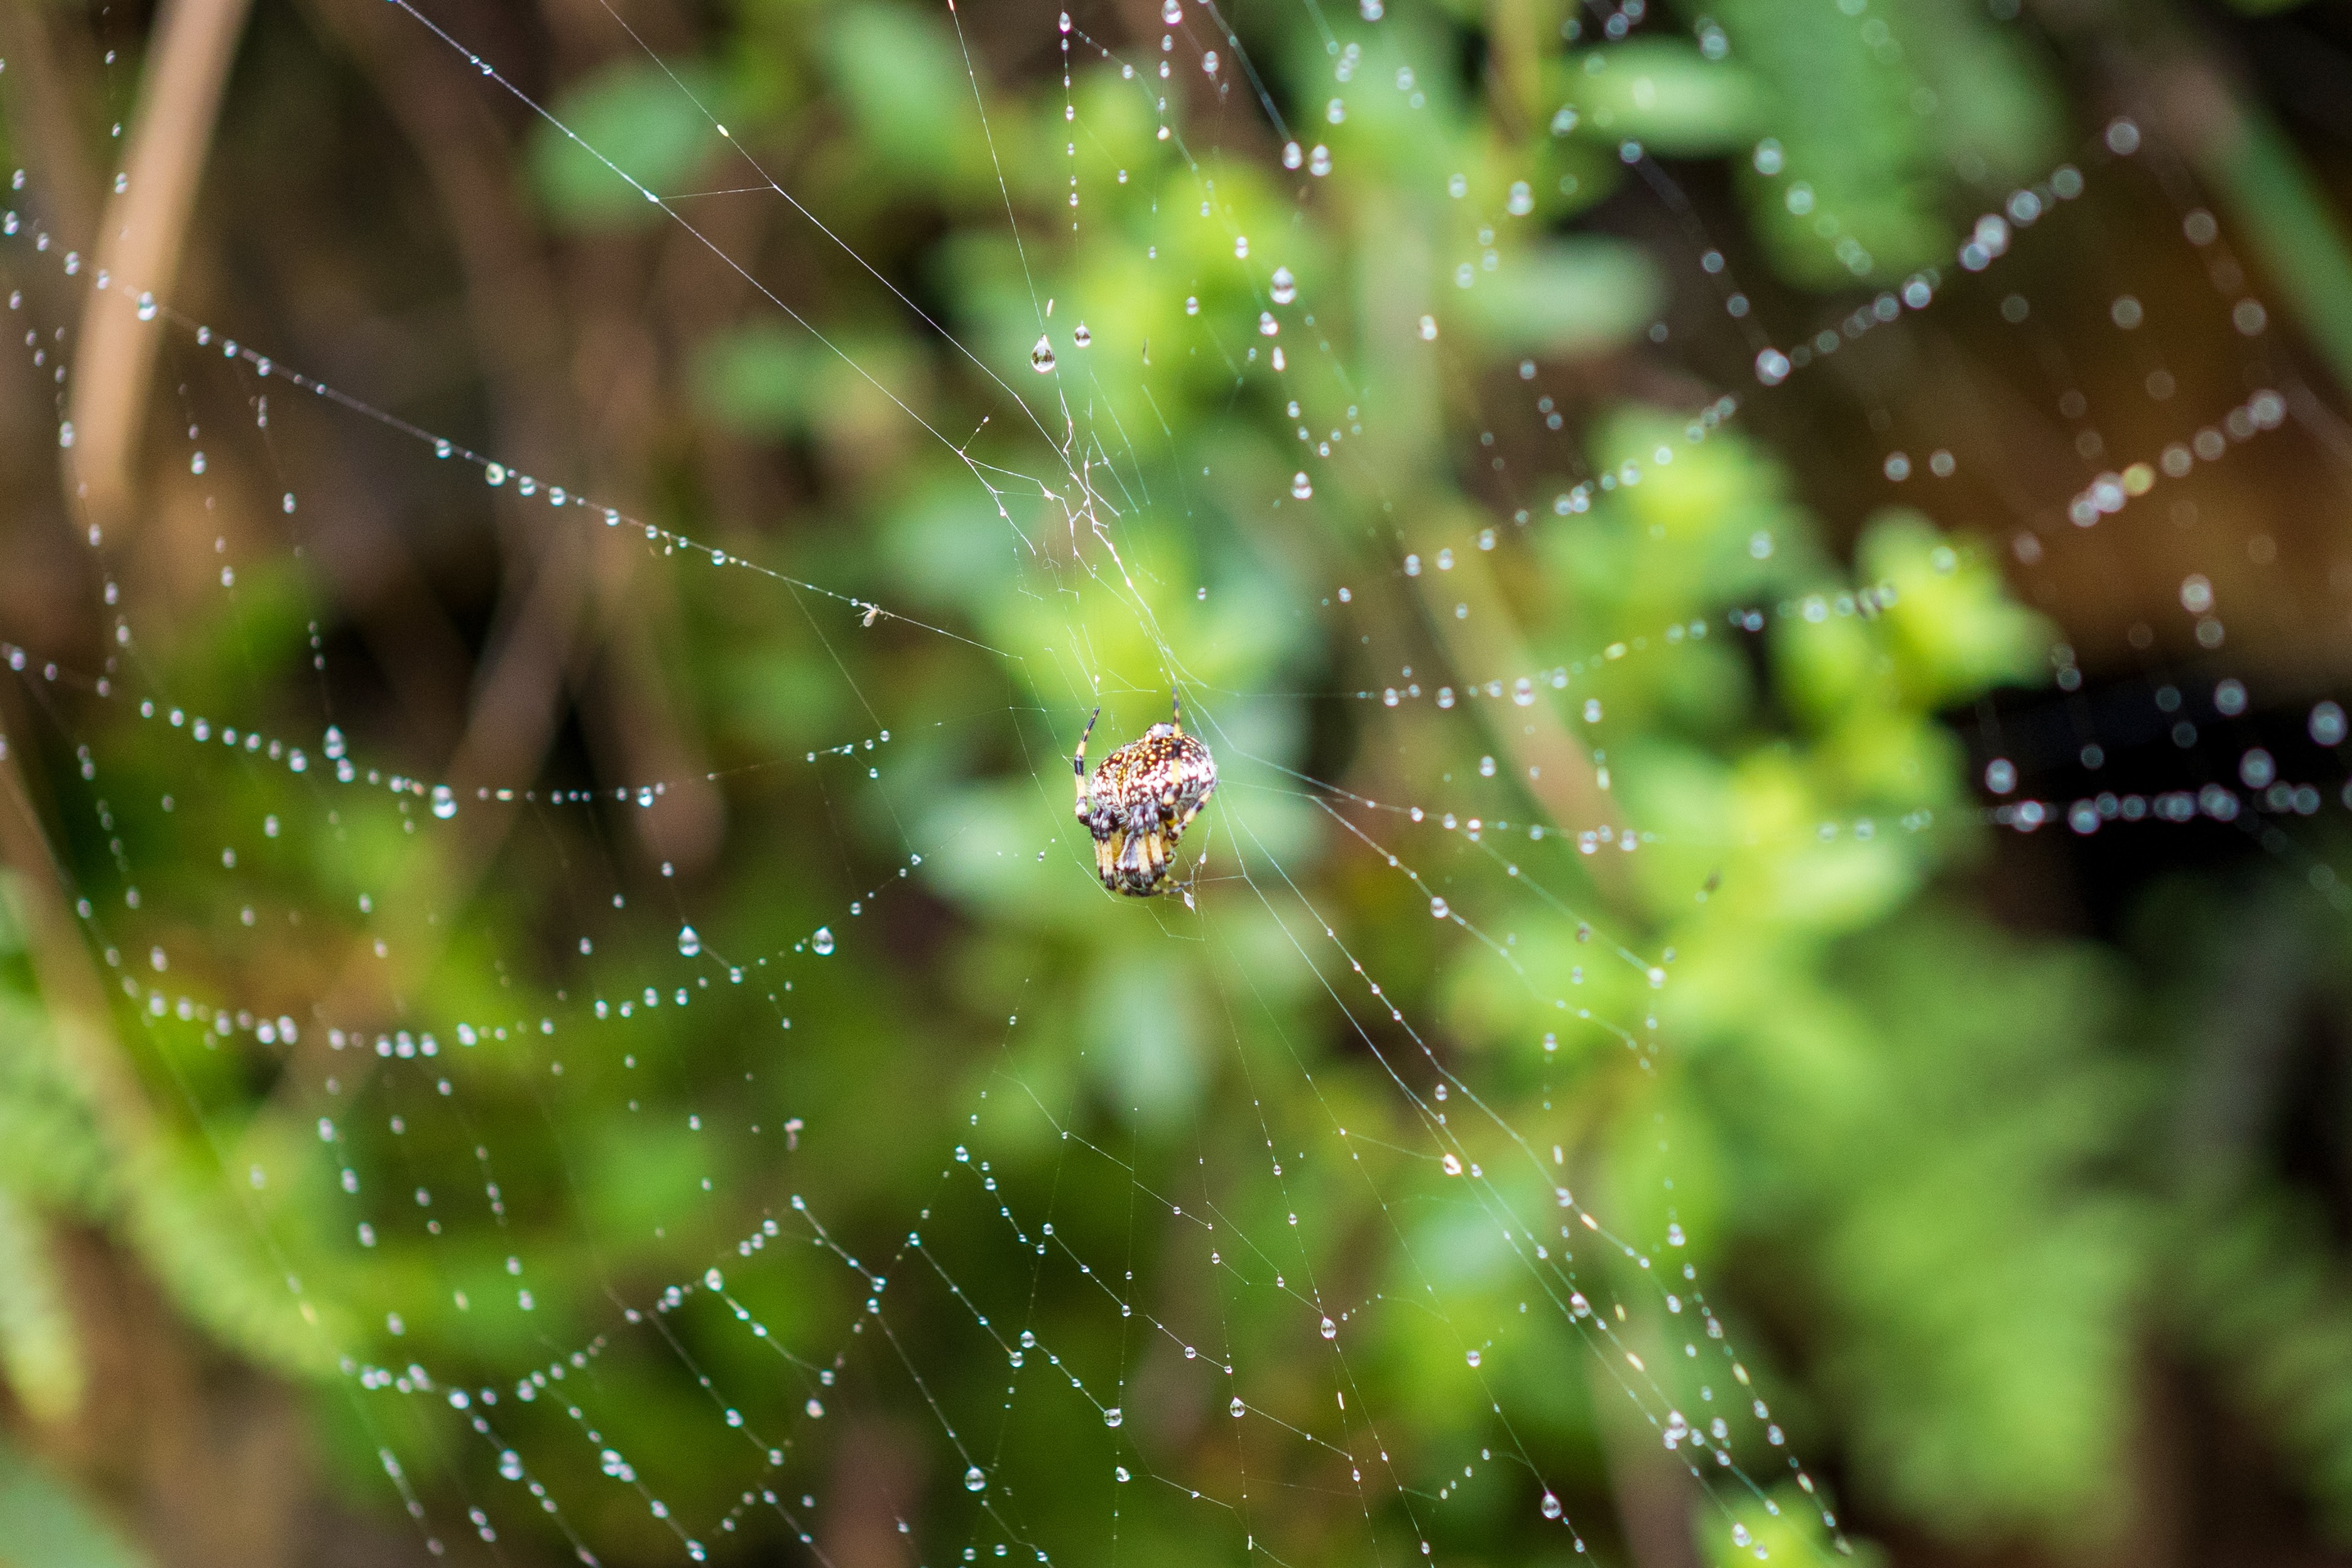
\includegraphics[width=\textwidth]{img/IMG_5321.jpeg}
      \fuentefigura{Fotografía de autoría propia; Bosques de Milpa Alta.}
    \end{column}
    \begin{column}{0.39\textwidth}
      \small
      {\itshape\color{ColorPrincipal}
        «una tendencia a concentrarse en profundidad con exclusión de otros
        estímulos»\par}
      {\raggedleft\footnotesize\color{gray!70} --- \citet[p.~34]{wood2021}\par}

      \vspace{0.3cm}
      {\itshape\color{ColorPrincipal}
        «durante un estado de hiperfoco hay una percepción disminuida de los
        estímulos no relevantes para la tarea»\par}
      {\raggedleft\footnotesize\color{gray!70} --- \citet{ashinoff2021}\par}

      \vspace{0.3cm}
      % EDITAR: explicación propuesta (redacción propia).
      La araña queda nítida; el resto de la escena sigue ahí, pero pierde
      definición.
    \end{column}
  \end{columns}
\end{frame}

% ── Frame: Hiperfoco, ejemplo 2 (el entorno se vuelve luces difusas) ─────────
\begin{frame}{Hiperfoco: el entorno se vuelve luces difusas}
  \begin{columns}[c,totalwidth=\textwidth]
    \begin{column}{0.58\textwidth}
      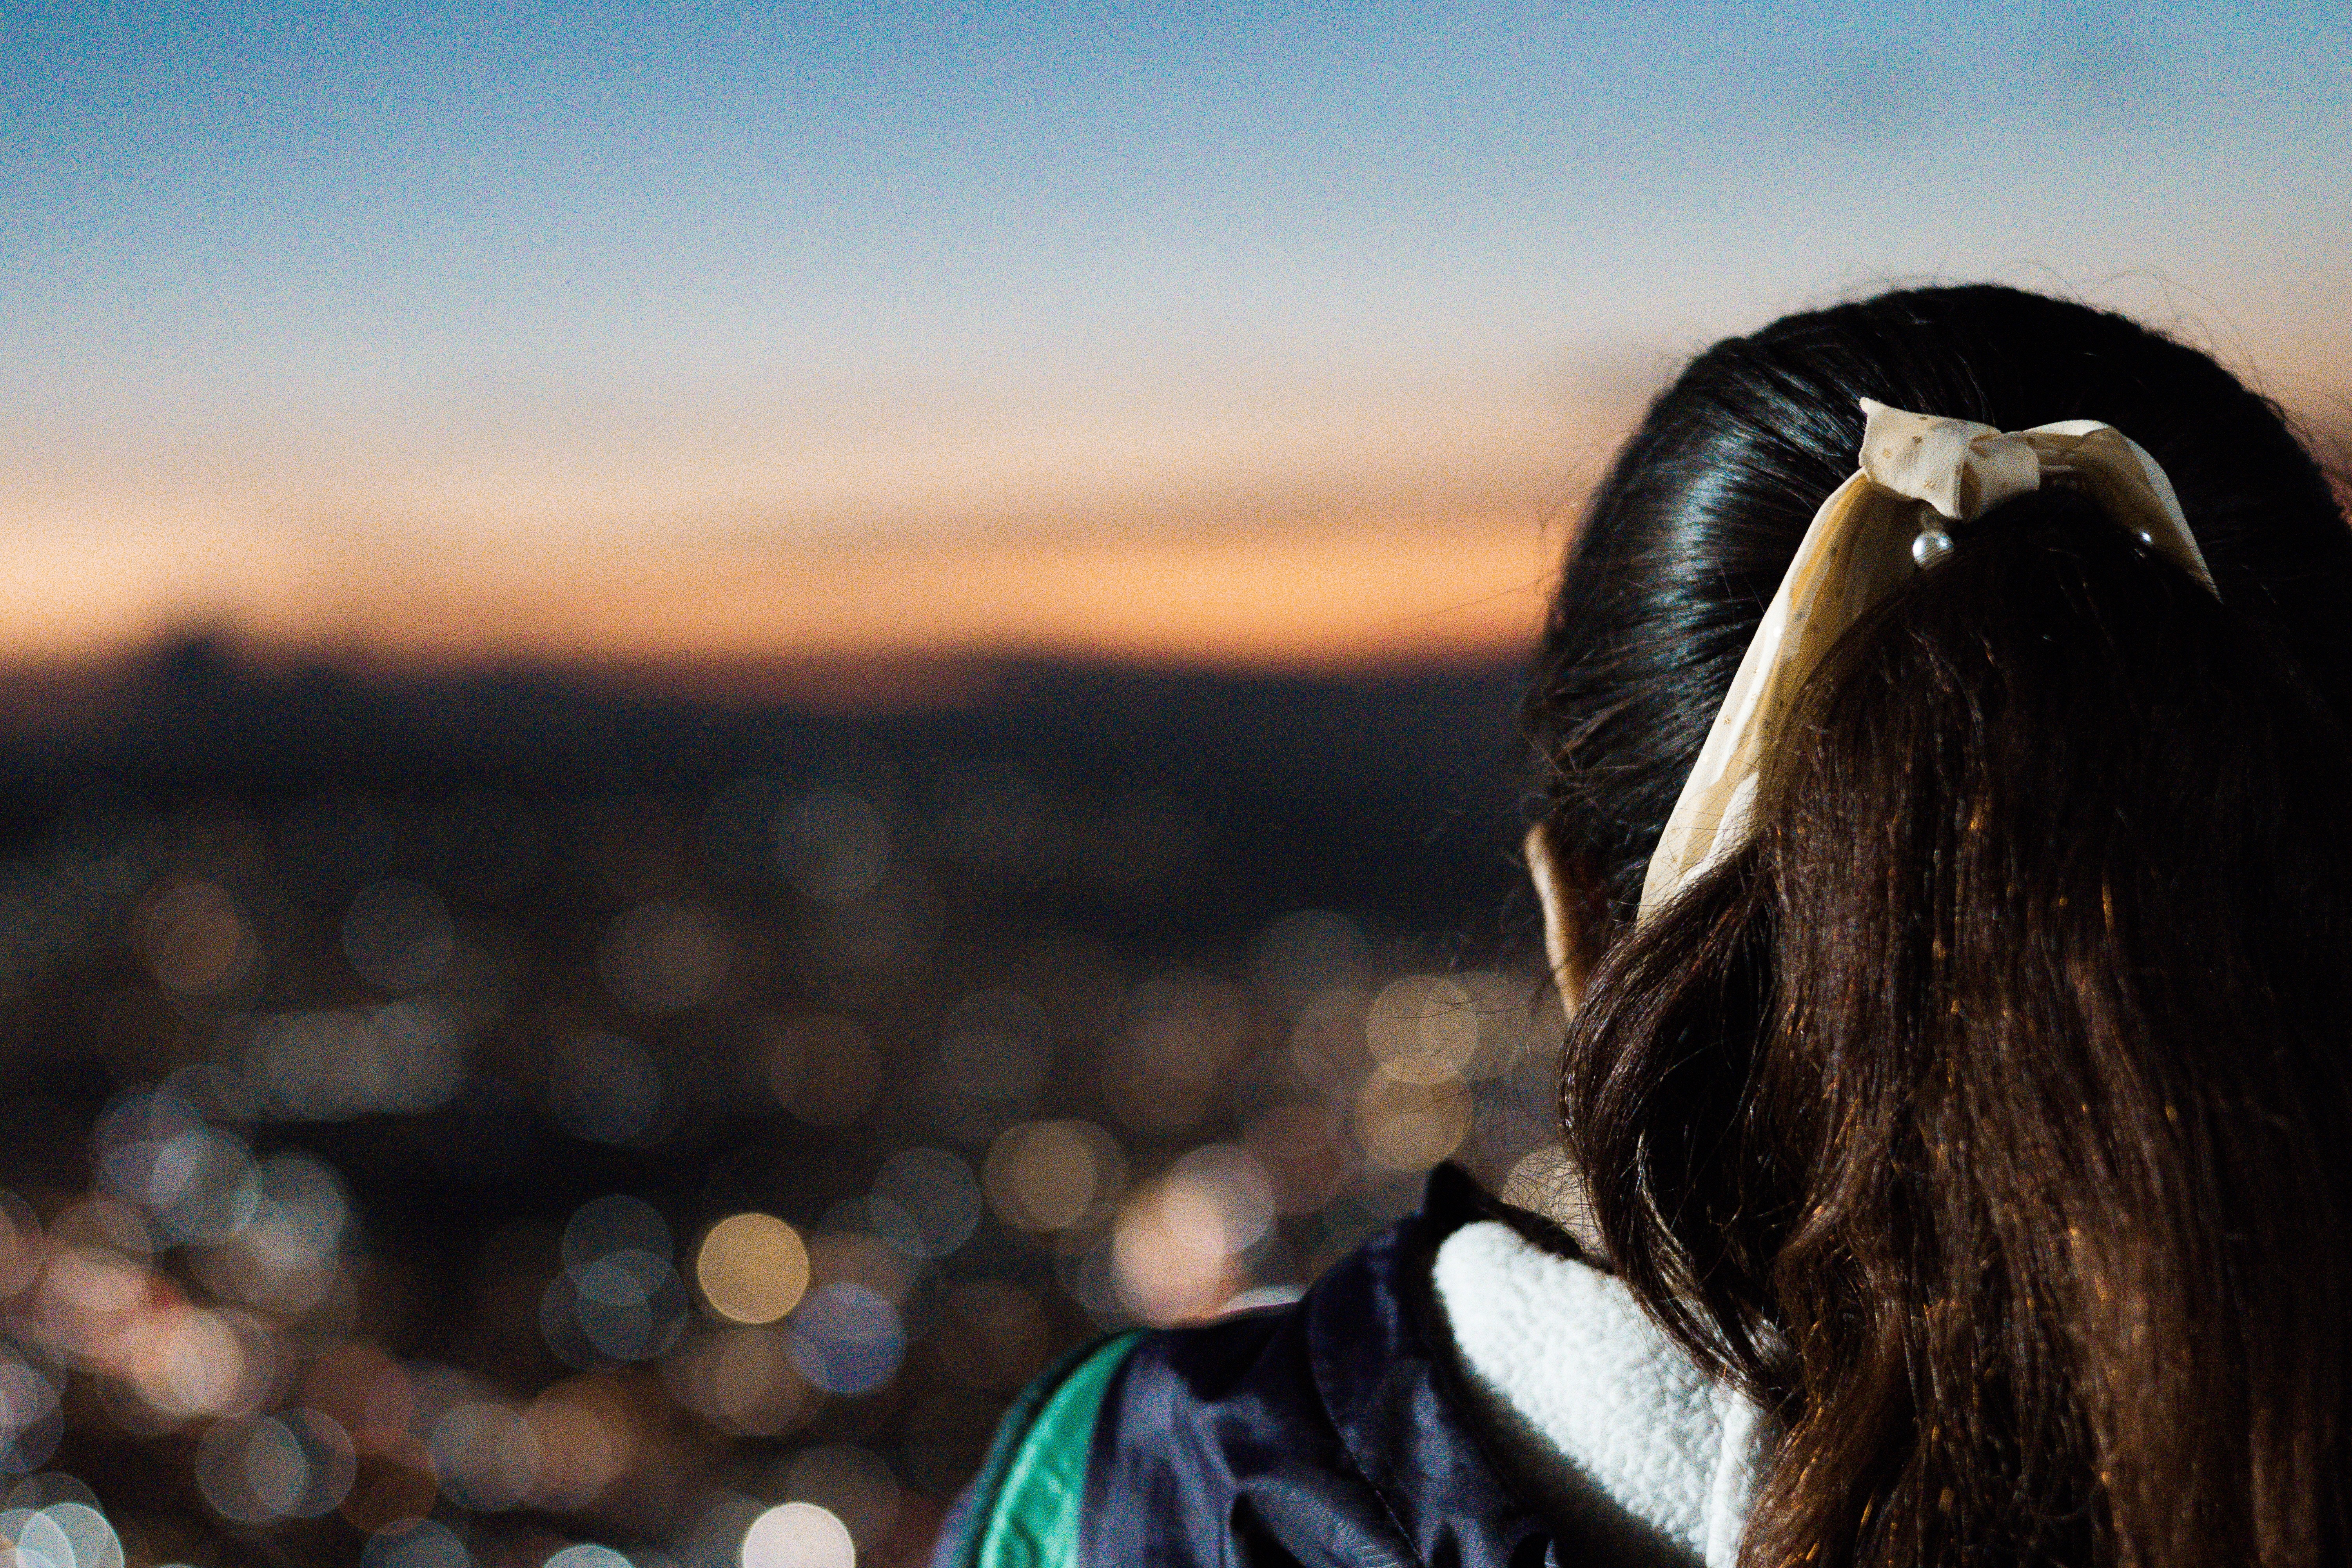
\includegraphics[width=\textwidth]{img/IMG_5357.jpeg}
      \fuentefigura{Fotografía de autoría propia; Catedral de Sal Zipaquirá en Colombia.}
      % EDITAR: autoría o fuente de la fotografía.
    \end{column}
    \begin{column}{0.39\textwidth}
      \small
      {\itshape\color{ColorPrincipal}
        «durante un estado de hiperfoco, el desempeño en la tarea mejora»\par}
      {\raggedleft\footnotesize\color{gray!70} --- \citet{ashinoff2021}\par}

      \vspace{0.3cm}
      {\itshape\color{ColorPrincipal}
        «la importancia de percibir esta disposición como una fortaleza, en
        lugar de un déficit que deba remediarse de algún modo»\par}
      {\raggedleft\footnotesize\color{gray!70} --- \citet{wood2021}\par}

      \vspace{0.3cm}
      % EDITAR: explicación propuesta (redacción propia).
      La ciudad no desaparece: se convierte en luces difusas mientras la
      atención se queda en un solo punto.
    \end{column}
  \end{columns}
\end{frame}


% ── Diapositivas a pantalla completa ─────────────────────────────────────────
%  Las imágenes se leen de la guía (Articulo1), sin duplicarlas.
%  \DiapositivaCompleta{ruta}{capa TikZ opcional}{nota del presentador}
%  Las notas (\note) no se proyectan; para verlas en una segunda pantalla:
%  \setbeameroption{show notes on second screen=right} en main.tex (pdfpc).
\providecommand{\RutaDinamicaTres}{../Articulo1/Resources/img/Dinamica3}
\providecommand{\DiapositivaCompleta}[3]{%
  {\setbeamertemplate{navigation symbols}{}% sin íconos de navegación
  \begin{frame}[plain]
    \begin{tikzpicture}[remember picture,overlay]
      \node at (current page.center)
        {\includegraphics[width=\paperwidth,height=\paperheight]{#1}};
      #2
    \end{tikzpicture}
    \note{#3}
  \end{frame}}}

% ── Frame: Antes de leer ─────────────────────────────────────────────────────
\begin{frame}{Antes de leer}
  \vfill
  \begin{center}
    {\Large\color{ColorPrincipal} Lean el texto e intenten retener los detalles.\par}
  \end{center}
  \vfill
  \note{Iniciar el audio (Audio\_Final\_Prueba.wav) desde 0:00 al pasar a la
  siguiente diapositiva.}
\end{frame}

% ── Fase 1: Odisea, Canto IX (audio 0:00 – 1:55, propuesta) ──────────────────
\DiapositivaCompleta{\RutaDinamicaTres/Fase1/Dinamica3_Fase1_Diapositiva1.png}{}
  {Audio 0:00 -- 1:55 (propuesta): base de oficina y pasillo. El grupo lee e
  intenta retener los detalles.}

\DiapositivaCompleta{\RutaDinamicaTres/Fase1/Dinamica3_Fase1_Diapositiva2.png}{}
  {Explicar que el hiperfoco permite ignorar la paja o el adorno social y
  literario para ir directo al núcleo de la información.}

% EDITAR: texto guía sobre el audio (redacción propia).
\DiapositivaCompleta{\RutaDinamicaTres/Fase1/Dinamica3_Fase1_Diapositiva3.png}
  {\node[anchor=south, text=white!75!black, font=\scriptsize]
     at ([yshift=0.3cm]current page.south)
     {El audio continúa. La siguiente lectura comenzará en unos minutos.};}
  {Se queda proyectada hasta 4:52, cuando comienza la Fase 2.}

% =============================================================================
%  4-Dinamica-3.tex — Continuación directa de la inmersión: Rayuela, cap. 34
%  (hiperfoco ante un texto más complejo) y cap. 68 (meltdown), y el corte.
%  Usa \DiapositivaCompleta y \RutaDinamicaTres, definidos en 3-Dinamica-2.tex.
%  Intervalos de audio: propuesta de la guía (sección 4.5), pendientes de confirmar.
% =============================================================================

% ── Fase 2: Rayuela, cap. 34 (audio 4:52 – 10:34, punto medio) ───────────────
\DiapositivaCompleta{\RutaDinamicaTres/Fase2/Dinamica3_Fase2_Diapositiva1.png}{}
  {Audio 4:52 -- 10:34 (propuesta): punto medio. Pedir al grupo que lea el
  texto de corrido.}

\DiapositivaCompleta{\RutaDinamicaTres/Fase2/Dinamica3_Fase2_Diapositiva2.png}{}
  {Explicar que el filtro separa los dos hilos del texto y deja pasar solo el
  que interesa.}

\DiapositivaCompleta{\RutaDinamicaTres/Fase2/Dinamica3_Fase2_Diapositiva3.png}{}
  {El resumen evidencia el resultado del procesamiento analítico.}

% ── Fase 3: crisis (audio 10:34 – 13:57, punto alto) ─────────────────────────
\DiapositivaCompleta{\RutaDinamicaTres/Fase3/Dinamica3_Fase3_Diapositiva1.png}{}
  {FASE DE CRISIS. Audio 10:34 -- 13:57 (propuesta): punto alto, tinnitus
  agudo. Se proyecta de nuevo el resumen que el grupo ya comprendió.}

\DiapositivaCompleta{\RutaDinamicaTres/Fase3/Dinamica3_Fase3_Diapositiva2.png}{}
  {Crisis: luces agresivas y desenfoque severo; ya no hay capa nítida.}

% EDITAR: qué se proyecta durante la meseta final del audio (13:57 – 18:58).
\DiapositivaCompleta{\RutaDinamicaTres/Fase3/Dinamica3_Fase3_Diapositiva3.png}{}
  {Crisis: el quiebre al glíglico. Las letras se ven con claridad, pero el
  significado ya no llega.}

% ── Frame: Corte (pantalla en blanco) ────────────────────────────────────────
{\setbeamertemplate{navigation symbols}{}% sin íconos de navegación
\begin{frame}[plain]
  \begin{tikzpicture}[remember picture,overlay]
    \fill[white] (current page.south west) rectangle (current page.north east);
  \end{tikzpicture}
  \note{Cortar el audio de tajo y sustituirlo por ruido blanco. Explicar el
  shutdown.}
\end{frame}
}

\section{Conclusiones}

% ── Frame: Conexión con la teoría ────────────────────────────────────────────
% EDITAR: borrador propuesto. Citas tomadas de Articulo1/secciones/3-Conceptos.tex
%         (traducción propia; el original está en los % ORIG: de la guía).
\begin{frame}{Conexión con la teoría}
  % \begingroup en vez de {…}: un grupo tras el título Beamer lo toma como subtítulo.
  \begingroup\footnotesize
  \renewcommand{\arraystretch}{1.1}
  % Sin >{...}: babel-spanish vuelve activos < y >. Se usa \raggedright
  % en cada celda y \tabularnewline para cerrar renglones.
  \begin{tabularx}{\textwidth}{@{}p{0.30\textwidth}X@{}}
    \toprule
    \textbf{Lo que vivimos → concepto} & \textbf{Lo que dice la investigación} \tabularnewline
    \midrule
    \raggedright Dinámica 1: sostener la mirada y la conversación
    → \textbf{Masking}
      & \raggedright\enquote{El camuflaje fue descrito con frecuencia como algo mental, física y emocionalmente agotador} \citep{hull2017} \tabularnewline
    \raggedright Dinámica 2: un solo objeto nítido y el resto difuso
    → \textbf{Hiperfoco}
      & \raggedright\enquote{Durante un estado de hiperfoco hay una percepción disminuida de los estímulos no relevantes para la tarea} \citep{ashinoff2021} \tabularnewline
    \raggedright Dinámica 3: lectura con audio hasta la fase de crisis
    → \textbf{Meltdown / shutdown}
      & \raggedright Detonantes: \enquote{demandas sociales, frustración, vergüenza, dificultades de comunicación, detonantes emocionales y estímulos sensoriales aversivos abrumadores} \citep{phung2021} \tabularnewline
    \bottomrule
  \end{tabularx}
  \par\endgroup

  \begin{block}{Lo que une a las tres dinámicas}
    {\footnotesize
    El burnout autista surge de \enquote{los estresores de la vida (subtemas:
    enmascaramiento, expectativas, manejo de la discapacidad y cambios vitales)
    que conducen a una carga acumulada} \citep{raymaker2020}: la máscara de la
    Dinámica 1 también alimenta la crisis de la Dinámica 3.\par}
  \end{block}
\end{frame}

% ── Frame: Conclusiones ───────────────────────────────────────────────────────
\begin{frame}{Conclusiones: ¿cómo ayudo?}
  \begin{columns}[T]
    \begin{column}{0.48\textwidth}
      \begin{block}{Lo que ayuda}
        \footnotesize
        \begin{itemize}
          \item Entender que la normalidad no es una ley, sino un estereotipo no universal.
          \item No todas las discapacidades son visibles, ni todas las personas con discapacidad son dependientes.
          \item El término \enquote{inclusión} no solo se aplica a las personas con sexualidad diversa, sino a todas las que no encajan en la norma.
          \item La sinceridad y la claridad ante las diferencias pueden evitar la discriminación.
        \end{itemize}
      \end{block}
    \end{column}
    \begin{column}{0.48\textwidth}
      \begin{alertblock}{Lo que no ayuda}
        \footnotesize
        \begin{itemize}
          \item Usar frases como \enquote{Todos somos un poco autistas} o \enquote{Todos somos un poco discapacitados} para justificar la discriminación.
          \item Propiciar etiquetas o estereotipos que excluyan a las personas con discapacidad de actividades sociales, educativas o laborales.
          \item Creer que adaptar entornos es privilegiar a las personas con discapacidad.
          \item Los discursos políticos sin acciones.
        \end{itemize}
      \end{alertblock}
    \end{column}
  \end{columns}
\end{frame}

% ── Frame: Experiencias personales ───────────────────────────────────────────
\begin{frame}{Experiencias personales}
  \begin{columns}[T,onlytextwidth]
    \begin{column}{0.38\textwidth}
      \begin{block}{Médico}
        {\footnotesize\raggedright
        El reconocimiento médico en México es difícil, tortuoso y burocrático.
        Muchas personas con discapacidad no tienen acceso a un diagnóstico
        oficial y, por lo tanto, no pueden acceder a apoyos o servicios.
        Además, el personal médico no está capacitado para identificar a
        personas con trastorno del espectro autista, y muchas veces se les
        etiqueta como personas con problemas de conducta o de aprendizaje.\par}
      \end{block}
    \end{column}
    \begin{column}{0.29\textwidth}
      \begin{block}{Social}
        {\footnotesize\raggedright
        La libertad de creencia da a los demás la posibilidad de aceptar o no
        a las personas con discapacidad. En la mayoría de los casos, la gente
        se aleja cuando te percibe diferente: se te cataloga como una persona
        rara y se te excluye de actividades sociales.\par}
      \end{block}
    \end{column}
    \begin{column}{0.29\textwidth}
      \begin{block}{Laboral-Educativo}
        {\footnotesize\raggedright
        Un diagnóstico médico no garantiza la inclusión laboral o educativa.
        La discriminación es un problema estructural que se manifiesta en la
        falta de oportunidades, la exclusión de actividades y la
        estigmatización de las personas con discapacidad.\par}
      \end{block}
    \end{column}
  \end{columns}
\end{frame}


% ── Frame: Cierre ────────────────────────────────────────────────────────────
\begin{frame}[plain]
  \begin{center}
    \vfill
    {\color{ColorAcento}\rule{0.6\textwidth}{1.5pt}}\\[0.5cm]
    {\Large\bfseries\color{ColorPrincipal} Gracias}\\[0.3cm]
    {\normalsize \Autor}\\[0.1cm]
    {\small \MateriaCorta}\\[0.1cm]
    {\small \Semestre}\\[0.5cm]
    {\color{ColorAcento}\rule{0.6\textwidth}{1.5pt}}
    \vfill
  \end{center}
\end{frame}


% ── Anexo (material extra: solo si hay tiempo o preguntas) ───────────────────
\appendix
% =============================================================================
%  5-1-Extra-Cierre.tex — ANEXO: suicidio y neurodivergencia (material extra)
% =============================================================================
%  Se trata como POSIBLE CONSECUENCIA ASOCIADA a la sobrecarga (masking,
%  burnout, sobrecarga sensorial), no como causa ni como destino.
%  Citas: traducción propia; original en % ORIG:. Fuentes verificadas en
%  texto completo o resumen (PMC / Europe PMC / Crossref / editorial):
%    conner2023   PMC11042491 (manuscrito NIH)
%    septier2019  doi:10.1016/j.neubiorev.2019.05.022 (resumen)
%    sun2024      doi:10.1057/s41599-024-03578-1 (texto completo, acceso abierto)
%    moseley2024  doi:10.1089/aut.2022.0042 (resumen)
%    cassidy2018  doi:10.1186/s13229-018-0226-4 (resumen)
%  DESCARTADO del prompt por no poder verificarse textualmente:
%    «hasta 10 veces más en mujeres», «20.39 %», «3 a 5 veces» (Psychology
%    Today), «indefensión aprendida frente a reactividad», «exponencialmente».
%  Pautas: sin métodos, sin sensacionalismo; Línea de la Vida al inicio y al final.
% =============================================================================

\section{Anexo: suicidio y neurodivergencia}

% ── Frame: Aviso de contenido ────────────────────────────────────────────────
\begin{frame}{Antes de continuar: aviso de contenido}
  \begin{alertblock}{Este anexo habla de suicidio}
    \small
    Se presenta como material extra y con datos de investigación. El suicidio
    se aborda como una \textbf{posible consecuencia asociada} a la sobrecarga
    que vivimos en las dinámicas, no como un destino de las personas autistas
    o con TDAH.
  \end{alertblock}

  \vspace{0.4cm}
  \begin{block}{Si tú o alguien cercano lo necesita}
    \centering
    {\Large\bfseries\color{ColorPrincipal} Línea de la Vida: 800 911 2000}\par
    \vspace{0.1cm}
    {\small Gratuita, confidencial, las 24 horas, todos los días.}\par
  \end{block}
\end{frame}

% ── Frame: ¿Por qué hablar de esto? ──────────────────────────────────────────
\begin{frame}{¿Por qué hablar de esto?}
  \begin{block}{Un riesgo que pasa desapercibido}
    \small
    \enquote{Los últimos años de investigación nos han enseñado que las personas
    autistas tienen más probabilidad de morir por suicidio que las personas no
    autistas} \citep{conner2023}.
    % ORIG: The past several years of research have taught us that autistic
    %       people are more likely to die from suicide than non-autistic people.
  \end{block}

  \begin{block}{Lo que ya vivimos hoy}
    \small
    \enquote{La investigación ha mostrado que existen factores de riesgo y de
    protección potencialmente propios de las conductas y pensamientos suicidas
    en personas autistas, como \textbf{enmascarar sus características autistas},
    el \textbf{burnout autista} y la \textbf{sobrecarga sensorial}}
    \citep{conner2023}.
    % ORIG: research has shown that there are potentially unique risk and
    %       protective factors for suicidal thoughts and behaviors in autistic
    %       people, like masking their autism characteristics, autistic
    %       burnout, and sensory overload.
  \end{block}

  % EDITAR: frase puente (redacción propia).
  {\footnotesize\color{gray!80}
  Masking (Dinámica 1) y sobrecarga sensorial (Dinámica 3) aparecen aquí como
  factores de riesgo, no solo como experiencias incómodas.\par}
\end{frame}

% ── Frame: Autismo (gráfica) ─────────────────────────────────────────────────
\begin{frame}{Autismo: ideación e intentos en el último año}
  \begin{columns}[T,onlytextwidth]
    \begin{column}{0.56\textwidth}
      \centering
      % Escala: 1 % = 0.078 cm. Datos: Conner et al. (2023).
      \begin{tikzpicture}[x=1cm,y=0.078cm,font=\scriptsize]
        \draw[gray!60] (0,0) -- (6.4,0);
        % Jóvenes — ideación
        \fill[ColorPrincipal] (0.3,0) rectangle (0.8,20);
        \fill[gray!50]        (0.8,0) rectangle (1.3,14.2);
        \node[above] at (0.55,20)   {20};
        \node[above] at (1.05,14.2) {14.2};
        % Jóvenes — intentos
        \fill[ColorPrincipal] (1.7,0) rectangle (2.2,10);
        \fill[gray!50]        (2.2,0) rectangle (2.7,4.5);
        \node[above] at (1.95,10)  {10};
        \node[above] at (2.45,4.5) {4.5};
        % Adultos — ideación
        \fill[ColorPrincipal] (3.7,0) rectangle (4.2,42);
        \fill[gray!50]        (4.2,0) rectangle (4.7,4.8);
        \node[above] at (3.95,42)  {42};
        \node[above] at (4.45,4.8) {4.8};
        % Adultos — intentos
        \fill[ColorPrincipal] (5.1,0) rectangle (5.6,18);
        \fill[gray!50]        (5.6,0) rectangle (6.1,0.7);
        \node[above] at (5.35,18)  {18};
        \node[above] at (5.85,0.7) {0.7};
        % Etiquetas
        \node[below,align=center] at (0.8,0) {Ideación};
        \node[below,align=center] at (2.2,0) {Intentos};
        \node[below,align=center] at (4.2,0) {Ideación};
        \node[below,align=center] at (5.6,0) {Intentos};
        \node[font=\footnotesize\bfseries] at (1.5,-9) {Niñez y adolescencia};
        \node[font=\footnotesize\bfseries] at (4.9,-9) {Adultez};
        % Leyenda
        \fill[ColorPrincipal] (0.3,52) rectangle (0.55,55);
        \node[right] at (0.55,53.5) {Personas autistas};
        \fill[gray!50] (2.9,52) rectangle (3.15,55);
        \node[right] at (3.15,53.5) {Personas no autistas};
        \node[font=\tiny,gray] at (3.2,-14) {Porcentaje de personas en cada grupo};
      \end{tikzpicture}\par
      \vspace{0.1cm}
      {\tiny\itshape Fuente: elaboración propia con datos de \citet{conner2023}.\par}
    \end{column}
    \begin{column}{0.42\textwidth}
      \begin{block}{Diagnóstico en la adultez}
        \scriptsize
        \enquote{En estudios con personas que fueron diagnosticadas como autistas
        por primera vez en la adultez, más del 60\,\% reportó haber tenido
        ideación suicida} \citep{conner2023}.
        % ORIG: In studies of people who were first diagnosed as autistic in
        %       adulthood, over 60% reported having suicidal ideation.
      \end{block}
      \begin{alertblock}{Cómo leer la gráfica}
        \scriptsize
        Las cifras provienen de estudios distintos. Además, \enquote{muchos
        estudios han usado muestras en línea}, lo que podría elevar las tasas
        \citep{conner2023}.
        % ORIG: Many studies have used online samples, and it may be possible
        %       that relying on online studies may result in higher rates.
      \end{alertblock}
    \end{column}
  \end{columns}
\end{frame}

% ── Frame: TDAH y comorbilidad ───────────────────────────────────────────────
\begin{frame}{TDAH y la co-ocurrencia TEA + TDAH}
  \begin{columns}[T,onlytextwidth]
    \begin{column}{0.48\textwidth}
      \begin{block}{TDAH}
        \scriptsize
        Metaanálisis de 57 estudios: asociación significativa entre TDAH e
        \enquote{intentos de suicidio (2.37 \ldots), ideaciones suicidas
        (3.53 \ldots), planes suicidas (4.54 \ldots) y suicidio consumado
        (6.69 \ldots)}, en razón de momios \citep{septier2019}.
        % ORIG: we found a significant association between ADHD and suicidal
        %       attempts (2.37, 95% CI = 1.64-3.43; ...), suicidal ideations
        %       (3.53, 2.94-4.25; ...), suicidal plans (4.54, 2.46-8.37; ...),
        %       and completed suicide (6.69, 3.24-17.39; ...).

        \vspace{0.15cm}
        Un mecanismo posible es \enquote{la impulsividad, síntoma central bien
        establecido del TDAH}, junto con \enquote{déficits en las funciones
        ejecutivas implicadas en la regulación del control de impulsos y de las
        emociones} \citep{sun2024}.
        % ORIG: One of the possible underlying mechanisms might be, impulsivity,
        %       a well-established core symptom of ADHD [...]; and deficits in
        %       executive functions, that implicated in the regulation of
        %       impulse control and emotions, may further contribute to the
        %       suicidal behaviors
      \end{block}
    \end{column}
    \begin{column}{0.48\textwidth}
      \begin{block}{Rasgos TEA + TDAH}
        \scriptsize
        En 90\,882 universitarios (rasgos autorreportados, no diagnósticos), el
        riesgo fue \enquote{significativamente mayor en el grupo con rasgos de
        TDAH (OR = 1.24) y de TEA + TDAH (OR = 1.49)}; con rasgos de TEA solos
        no hubo diferencia frente al grupo control. El riesgo fue mayor en
        mujeres en los cuatro grupos \citep{sun2024}.
        % ORIG: Suicide risks were significantly higher in the ADHD (OR = 1.24,
        %       p < 0.001) and ASD + ADHD (OR = 1.49, p < 0.001) traits group.
        %       However, there was no significant difference in suicide risk
        %       between the ASD traits group (OR = 1.00, p = 1.00) and the
        %       control group. The risk of suicide was significantly higher for
        %       females than for males across all four groups (p < 0.001).
      \end{block}
      \begin{block}{¿Por qué?}
        \scriptsize
        En adultos autistas con probable TDAH, la suicidalidad podría
        relacionarse \enquote{con la percepción de ser una carga y con la
        capacidad suicida adquirida tras la exposición a eventos dolorosos y
        provocadores} \citep{moseley2024}.
        % ORIG: suicidality in autistic people with ADHD may be partially
        %       related to perceived burdensomeness and to acquired suicide
        %       capability after exposure to painful and provocative events.
      \end{block}
    \end{column}
  \end{columns}
\end{frame}

% ── Frame: Tabla comparativa ─────────────────────────────────────────────────
\begin{frame}{Resumen comparativo}
  % Sin >{...} en la especificación de columnas: babel-spanish activa < y >.
  \begingroup\scriptsize
  \renewcommand{\arraystretch}{1.05}
  \begin{tabularx}{\textwidth}{@{}p{0.17\textwidth}p{0.11\textwidth}p{0.11\textwidth}Xp{0.20\textwidth}@{}}
    \toprule
    \textbf{Población} & \textbf{Ideación} & \textbf{Intentos} & \textbf{Factores que señalan los autores} & \textbf{Medida y fuente} \tabularnewline
    \midrule
    \raggedright No autista, jóvenes & 14.2\,\% & 4.5\,\% & \raggedright ---
      & \raggedright Último año \citep{conner2023} \tabularnewline
    \raggedright No autista, adultos & 4.8\,\% & 0.7\,\% & \raggedright ---
      & \raggedright Último año \citep{conner2023} \tabularnewline
    \raggedright TEA, jóvenes & 20\,\% & 10\,\%
      & \raggedright Masking, burnout autista, sobrecarga sensorial
      & \raggedright Último año, metaanálisis \citep{conner2023} \tabularnewline
    \raggedright TEA, adultos & 42\,\% & 18\,\%
      & \raggedright Igual; con diagnóstico en la adultez, más del 60\,\% con ideación
      & \raggedright Último año \citep{conner2023} \tabularnewline
    \raggedright TDAH
      & OR 3.53
      & OR 2.37
      & \raggedright Impulsividad; funciones ejecutivas (control de impulsos y emociones)
      & \raggedright Metaanálisis, 57 estudios \citep{septier2019,sun2024} \tabularnewline
    \raggedright Rasgos TEA + TDAH
      & \multicolumn{2}{l}{Riesgo global: OR 1.49}
      & \raggedright Mayor riesgo en mujeres; percepción de ser una carga; eventos dolorosos
      & \raggedright Autorreporte, 90\,882 universitarios \citep{sun2024,moseley2024} \tabularnewline
    \bottomrule
  \end{tabularx}
  \par\endgroup

  \vspace{0.2cm}
  {\scriptsize\color{gray!80}
  OR (razón de momios): cuántas veces mayores son las probabilidades frente al
  grupo de comparación. Porcentajes y OR provienen de estudios y medidas
  distintas: no se suman ni se comparan directamente.\par}
\end{frame}

% ── Frame: El entorno como catalizador ───────────────────────────────────────
\begin{frame}{El entorno como catalizador}
  \begin{columns}[T,onlytextwidth]
    \begin{column}{0.48\textwidth}
      \begin{block}{Propios del autismo}
        \footnotesize
        \enquote{El camuflaje y las necesidades de apoyo no atendidas parecen
        ser marcadores de riesgo de suicidalidad propios de las condiciones del
        espectro autista} \citep{cassidy2018}.
        % ORIG: Camouflaging and unmet support needs appear to be risk markers
        %       for suicidality unique to ASC.
      \end{block}
      \begin{block}{Compartidos, pero más frecuentes}
        \footnotesize
        \enquote{La autolesión no suicida, el empleo y los problemas de salud
        mental parecen ser marcadores de riesgo compartidos con la población
        general, que son significativamente más prevalentes en la comunidad
        autista} \citep{cassidy2018}.
        % ORIG: Non-suicidal self-injury, employment, and mental health problems
        %       appear to be risk markers shared with the general population
        %       that are significantly more prevalent in the autistic community.
      \end{block}
    \end{column}
    \begin{column}{0.48\textwidth}
      \begin{block}{La respuesta de los demás}
        \footnotesize
        \enquote{A menudo las personas autistas viven la suicidalidad como una
        reacción a experiencias sociales negativas repetidas}
        \citep{conner2023}.
        % ORIG: often autistic people experience suicidality as a reaction to
        %       repeated negative social experiences.
      \end{block}
      \begin{alertblock}{Desde la experiencia personal}
        \footnotesize
        % EDITAR: el usuario redacta este bloque (sin cifras ni citas).
        El acoso escolar y la falta de diagnóstico se presentan aquí como una
        aproximación desde la experiencia personal, no como un dato
        estadístico.
      \end{alertblock}
    \end{column}
  \end{columns}
\end{frame}

% ── Frame: ¿Qué podemos hacer? ───────────────────────────────────────────────
\begin{frame}{¿Qué podemos hacer?}
  \begin{block}{Preguntar no hace daño}
    \small
    \enquote{Es importante preguntarle a la persona de forma clara y directa,
    con apoyo y sin castigo. Muchos años de investigación han mostrado que
    preguntar a las personas si han considerado el suicidio no las hace más
    propensas a tener pensamientos o conductas suicidas} \citep{conner2023}.
    % ORIG: it is important to ask the person clearly and directly, in a
    %       supportive and non-punitive manner. Many years of research has
    %       shown that asking people if they have considered suicide does not
    %       make them more likely to have suicidal thoughts or behaviors.
  \end{block}
  \begin{block}{Escuchar}
    \small
    \enquote{Escuchar y brindar apoyo y validación puede ser el primer y más
    importante paso} \citep{conner2023}.
    % ORIG: Listening and providing support and validation can be the first
    %       and most important step.
  \end{block}
  \vspace{0.1cm}
  {\centering\bfseries\color{ColorPrincipal} Línea de la Vida: 800 911 2000\par}
\end{frame}


% ── Bibliografía ─────────────────────────────────────────────────────────────
\section*{Referencias}
\begin{frame}[allowframebreaks]{Referencias}
  \bibliographystyle{apalike}
  \bibliography{referencias}
\end{frame}

\end{document}
